\documentclass[10pt]{beamer}
%\usepackage[catalan]{babel}
\usepackage[latin1]{inputenc}
\usepackage{times}
\usepackage{caption}
\usepackage[linesnumbered,ruled,vlined]{algorithm2e}
\usepackage{algpseudocode}
\usepackage{amssymb,amsthm,amsmath,epsfig,times,subfig,graphicx,tikz,multirow}
\usepackage{graphics,graphicx,makeidx}
\usepackage{xcolor}
\newtheorem{thm}{Theorem}
\newtheorem{lem}[thm]{Lemma}
\newtheorem{prop}[thm]{Proposition}
\newtheorem{cor}[thm]{Corollary}
\theoremstyle{definition}
\newtheorem{Def}{Definici�}
\newtheorem{rmk}{Remark}
\newtheorem{exam}{Example}


\usepackage{alphalph}
\renewcommand\thesubfigure{\alphalph{\value{subfigure}}}

\newcommand{\TM}{{T_{\text{M}}}}
\newcommand{\TNM}{{T_{\text{nM}}}}
\newcommand{\TP}{{T_{\text{P}}}}
\newcommand{\TLK}{{T_{\text{LK}}}}
\newcommand{\TD}{{T_{\text{D}}}}
\newcommand{\TSS}[1][]{T_{#1}^{\text{SS}}}



\newcommand{\SM}{{S_{\text{M}}}}
\newcommand{\SNM}{{S_{\text{nM}}}}
\newcommand{\SP}{{S_{\text{P}}}}
\newcommand{\SL}{{S_{\text{L}}}}
\newcommand{\SD}{{S_{\text{D}}}}
\newcommand{\SSS}[1][]{S_{#1}^{\text{SS}}}


\newcommand{\ILK}{{I_{\text{LK}}}}
\newcommand{\IKD}{{I_{\text{KD}}}}
\newcommand{\IRC}{{I_{\text{RC}}}}
\newcommand{\IYG}{{T_{\text{YG}}}}
\newcommand{\IGD}{{I_{\text{GD}}}}

\mode<presentation>
{
\usetheme{CambridgeUS}
%\setbeamercovered{transparent}
%\useinnertheme[shadow]{rounded}
\usecolortheme{orchid}
}



\title[TFM]{Visual people tracking with deep learning detection and feature tracking}
\author[M. Pieras]{%
  Author: Marcos Pieras Sagardoy\\ \vspace{0.25cm}
  Tutor: Jos� Mar�a Ca�as Plaza
}
\institute[UIB]{
 
\includegraphics[scale=0.2]{logo.jpg}
 }


\AtBeginSection[]
{
  \begin{frame}<beamer>
\begin{center}
\Large \textbf{\insertsection}
\end{center}
  \end{frame}
}

\begin{document}

\let\newblock\relax
\begin{frame}
  \titlepage
\end{frame}

\begin{frame}
  \frametitle{Index}
  \tableofcontents
\end{frame}


\section{Introduction}


\begin{frame}{Introduction}


\begin{Def}{Object tracking: }
Estimate the target state over time from image sequences
\end{Def}

\vspace{0.75cm}

It is challenging field due to:

\begin{itemize}


\item Variations beacause of geometric changes.

\item Variations due to photometric factors.

\item Occlusions.

\item Similar objects in the scene.


\end{itemize}




\end{frame}



\begin{frame}{Applications}



\begin{figure}[htbp]
\centering
\begin{tabular}{cc}

\subfloat[Surveillance ]{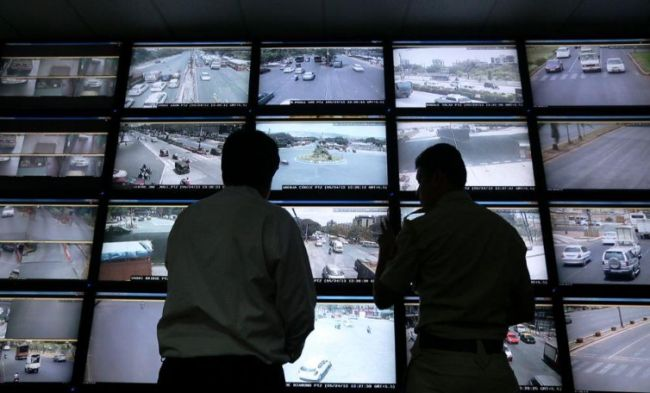
\includegraphics[width=40mm]{./aplicaciones/policias.jpg}}&
\subfloat[Sports]{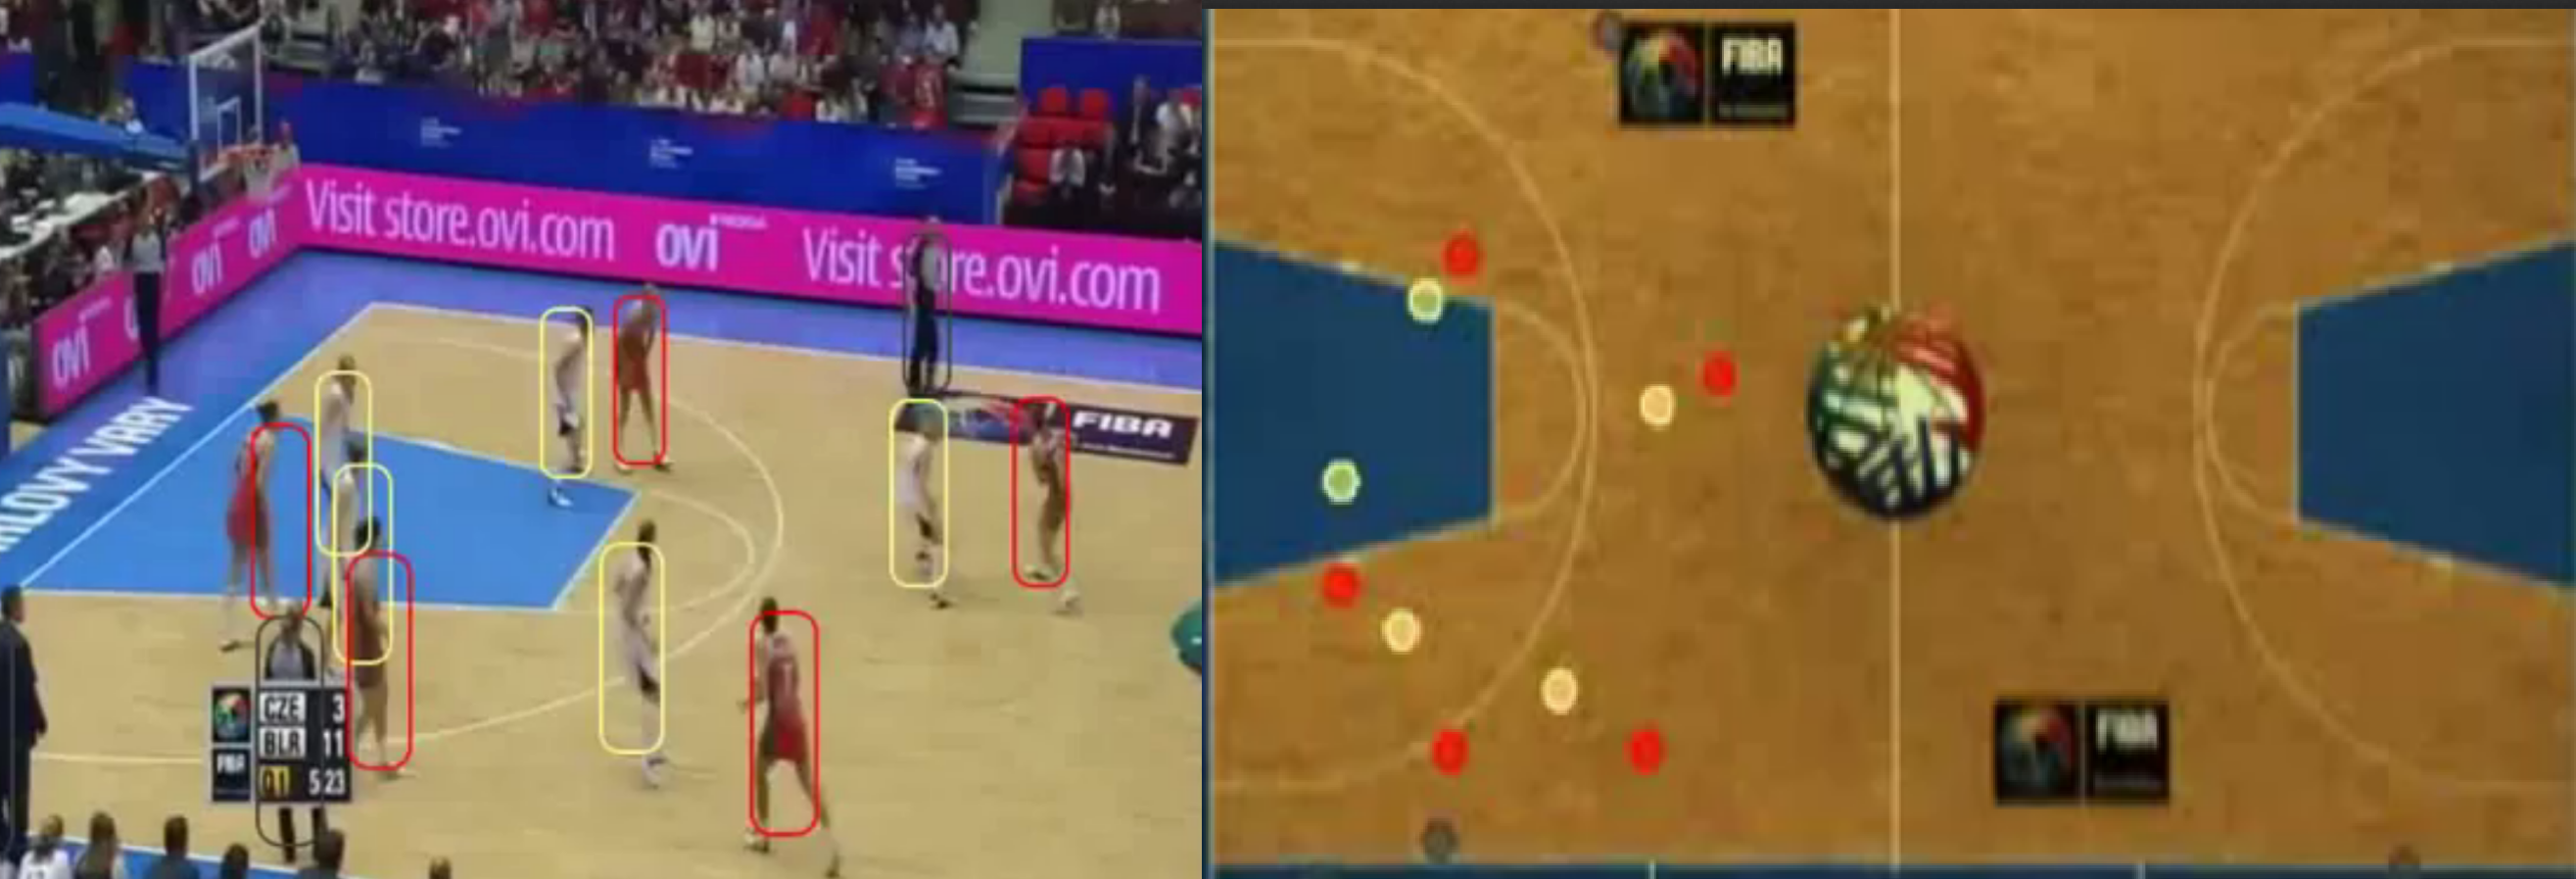
\includegraphics[width=40mm]{./aplicaciones/tomeu.png}}\\
\subfloat[Science]{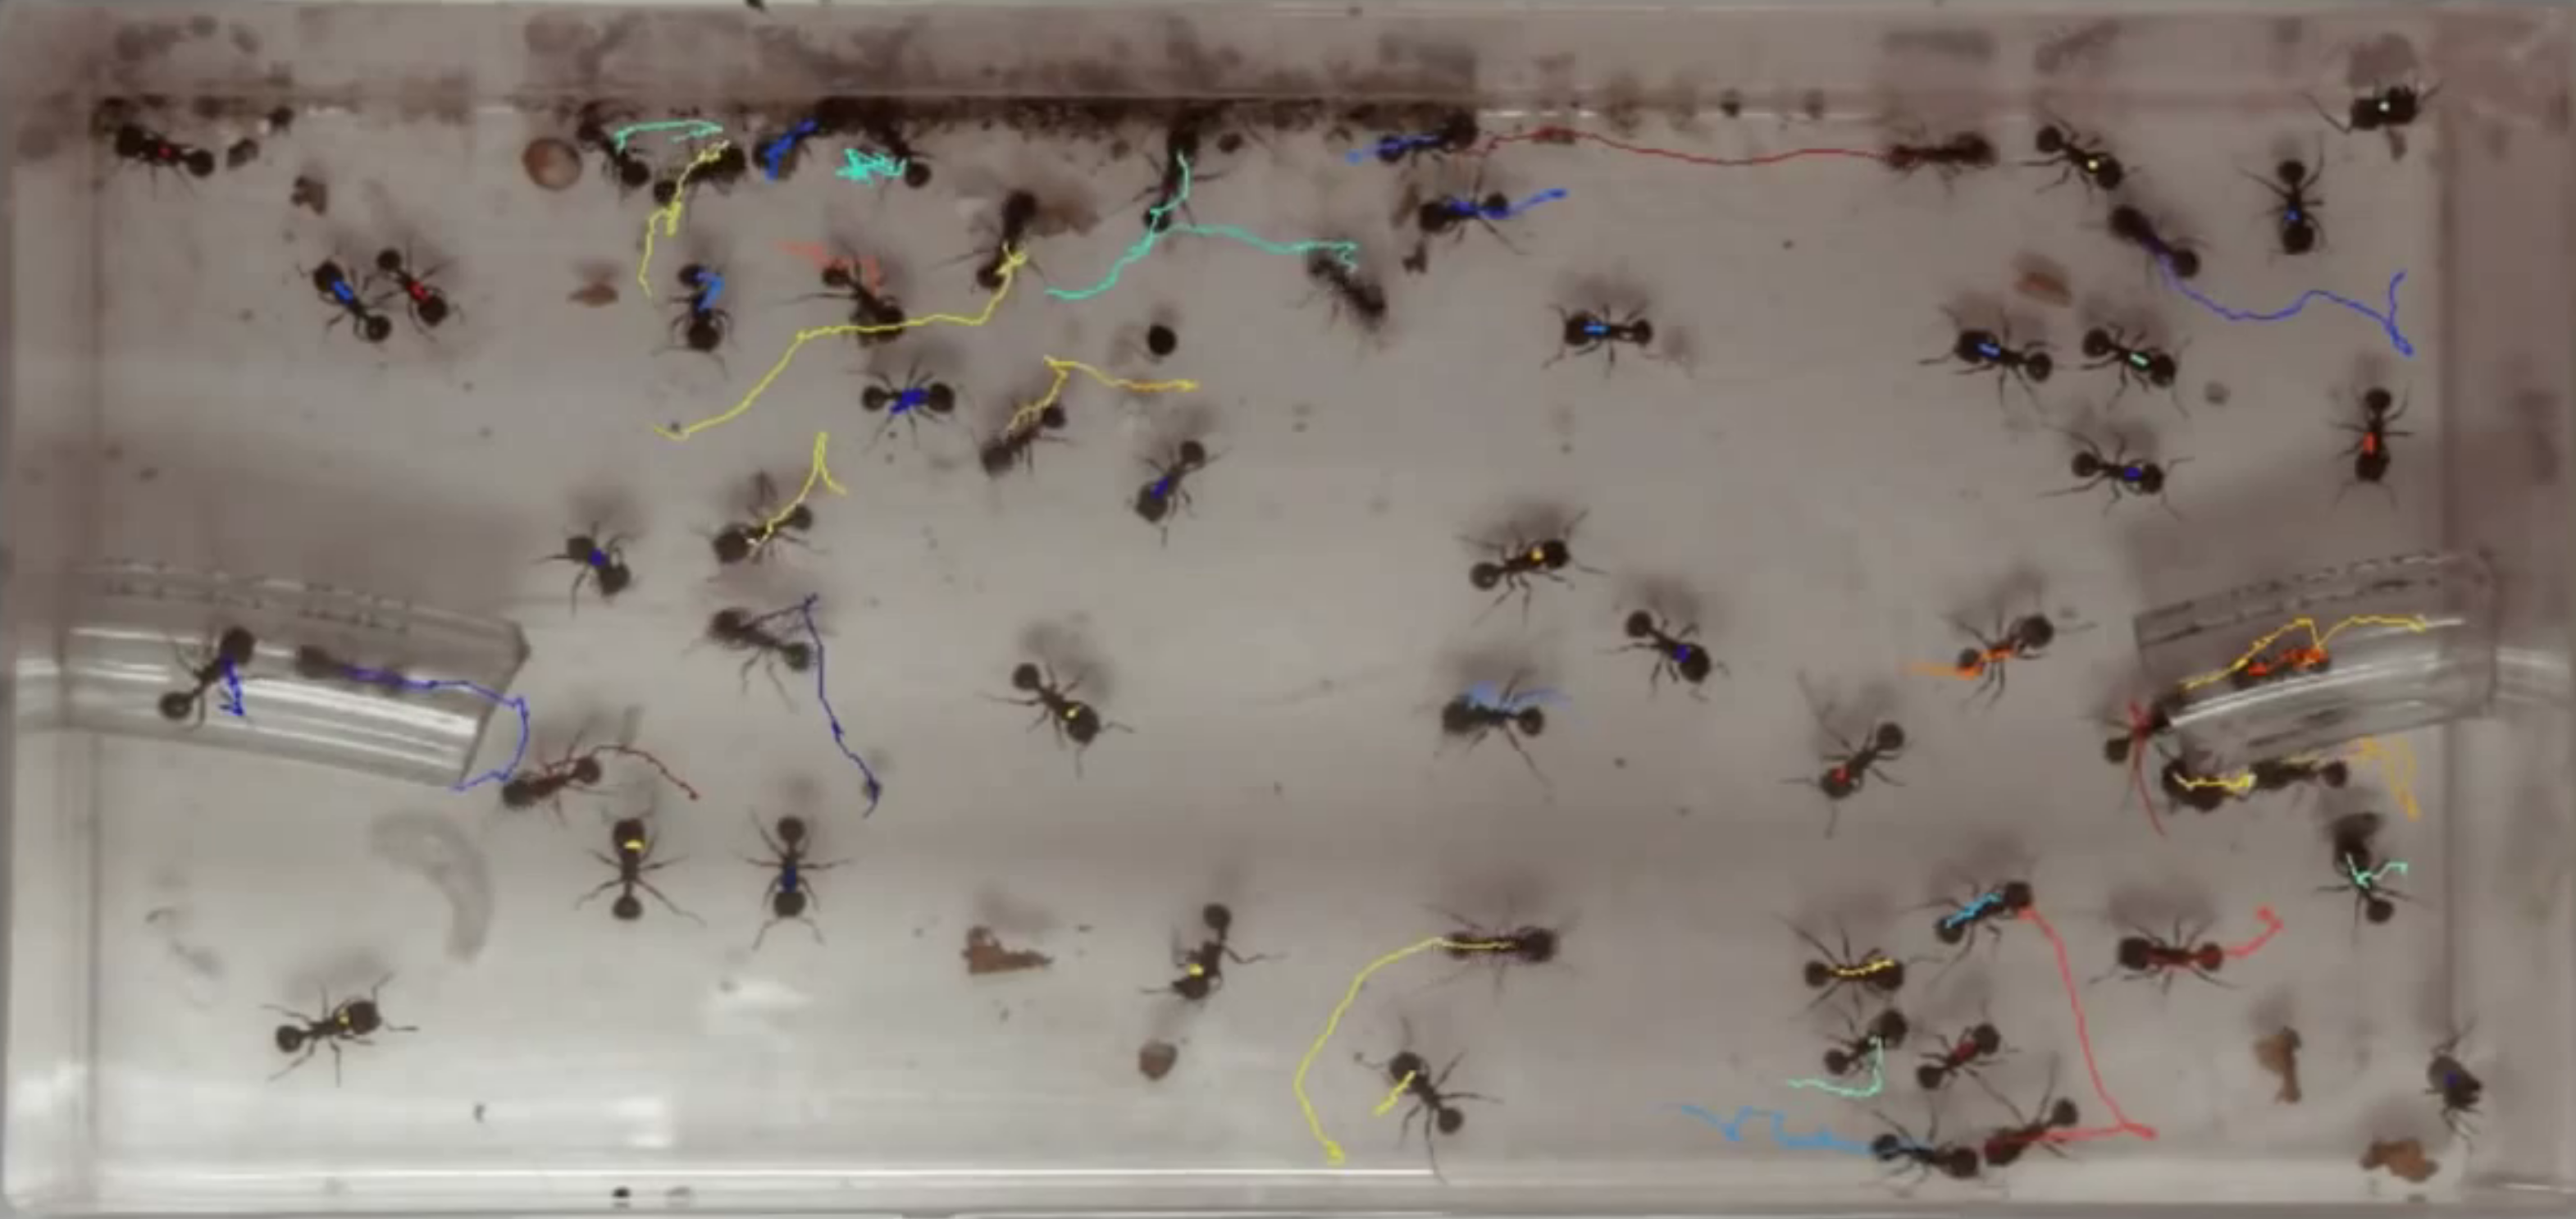
\includegraphics[width=40mm]{./aplicaciones/Seleccio_007.png}}&
\subfloat[Art]{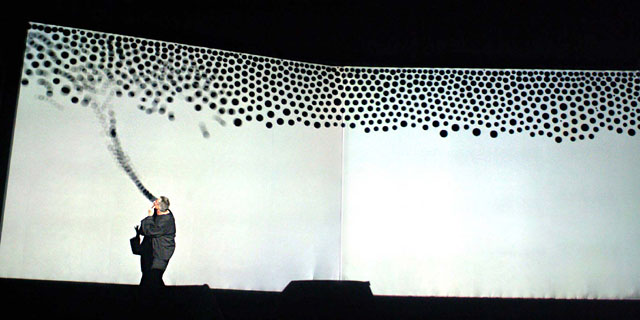
\includegraphics[width=40mm]{./aplicaciones/singing.jpg}}\\


\end{tabular}
%\caption{Imatges MRI amb tumor.} \label{pseudo}
\end{figure}


\end{frame}



\begin{frame}{Why deep learning techniques ?}


\begin{figure}[htbp]
\centering
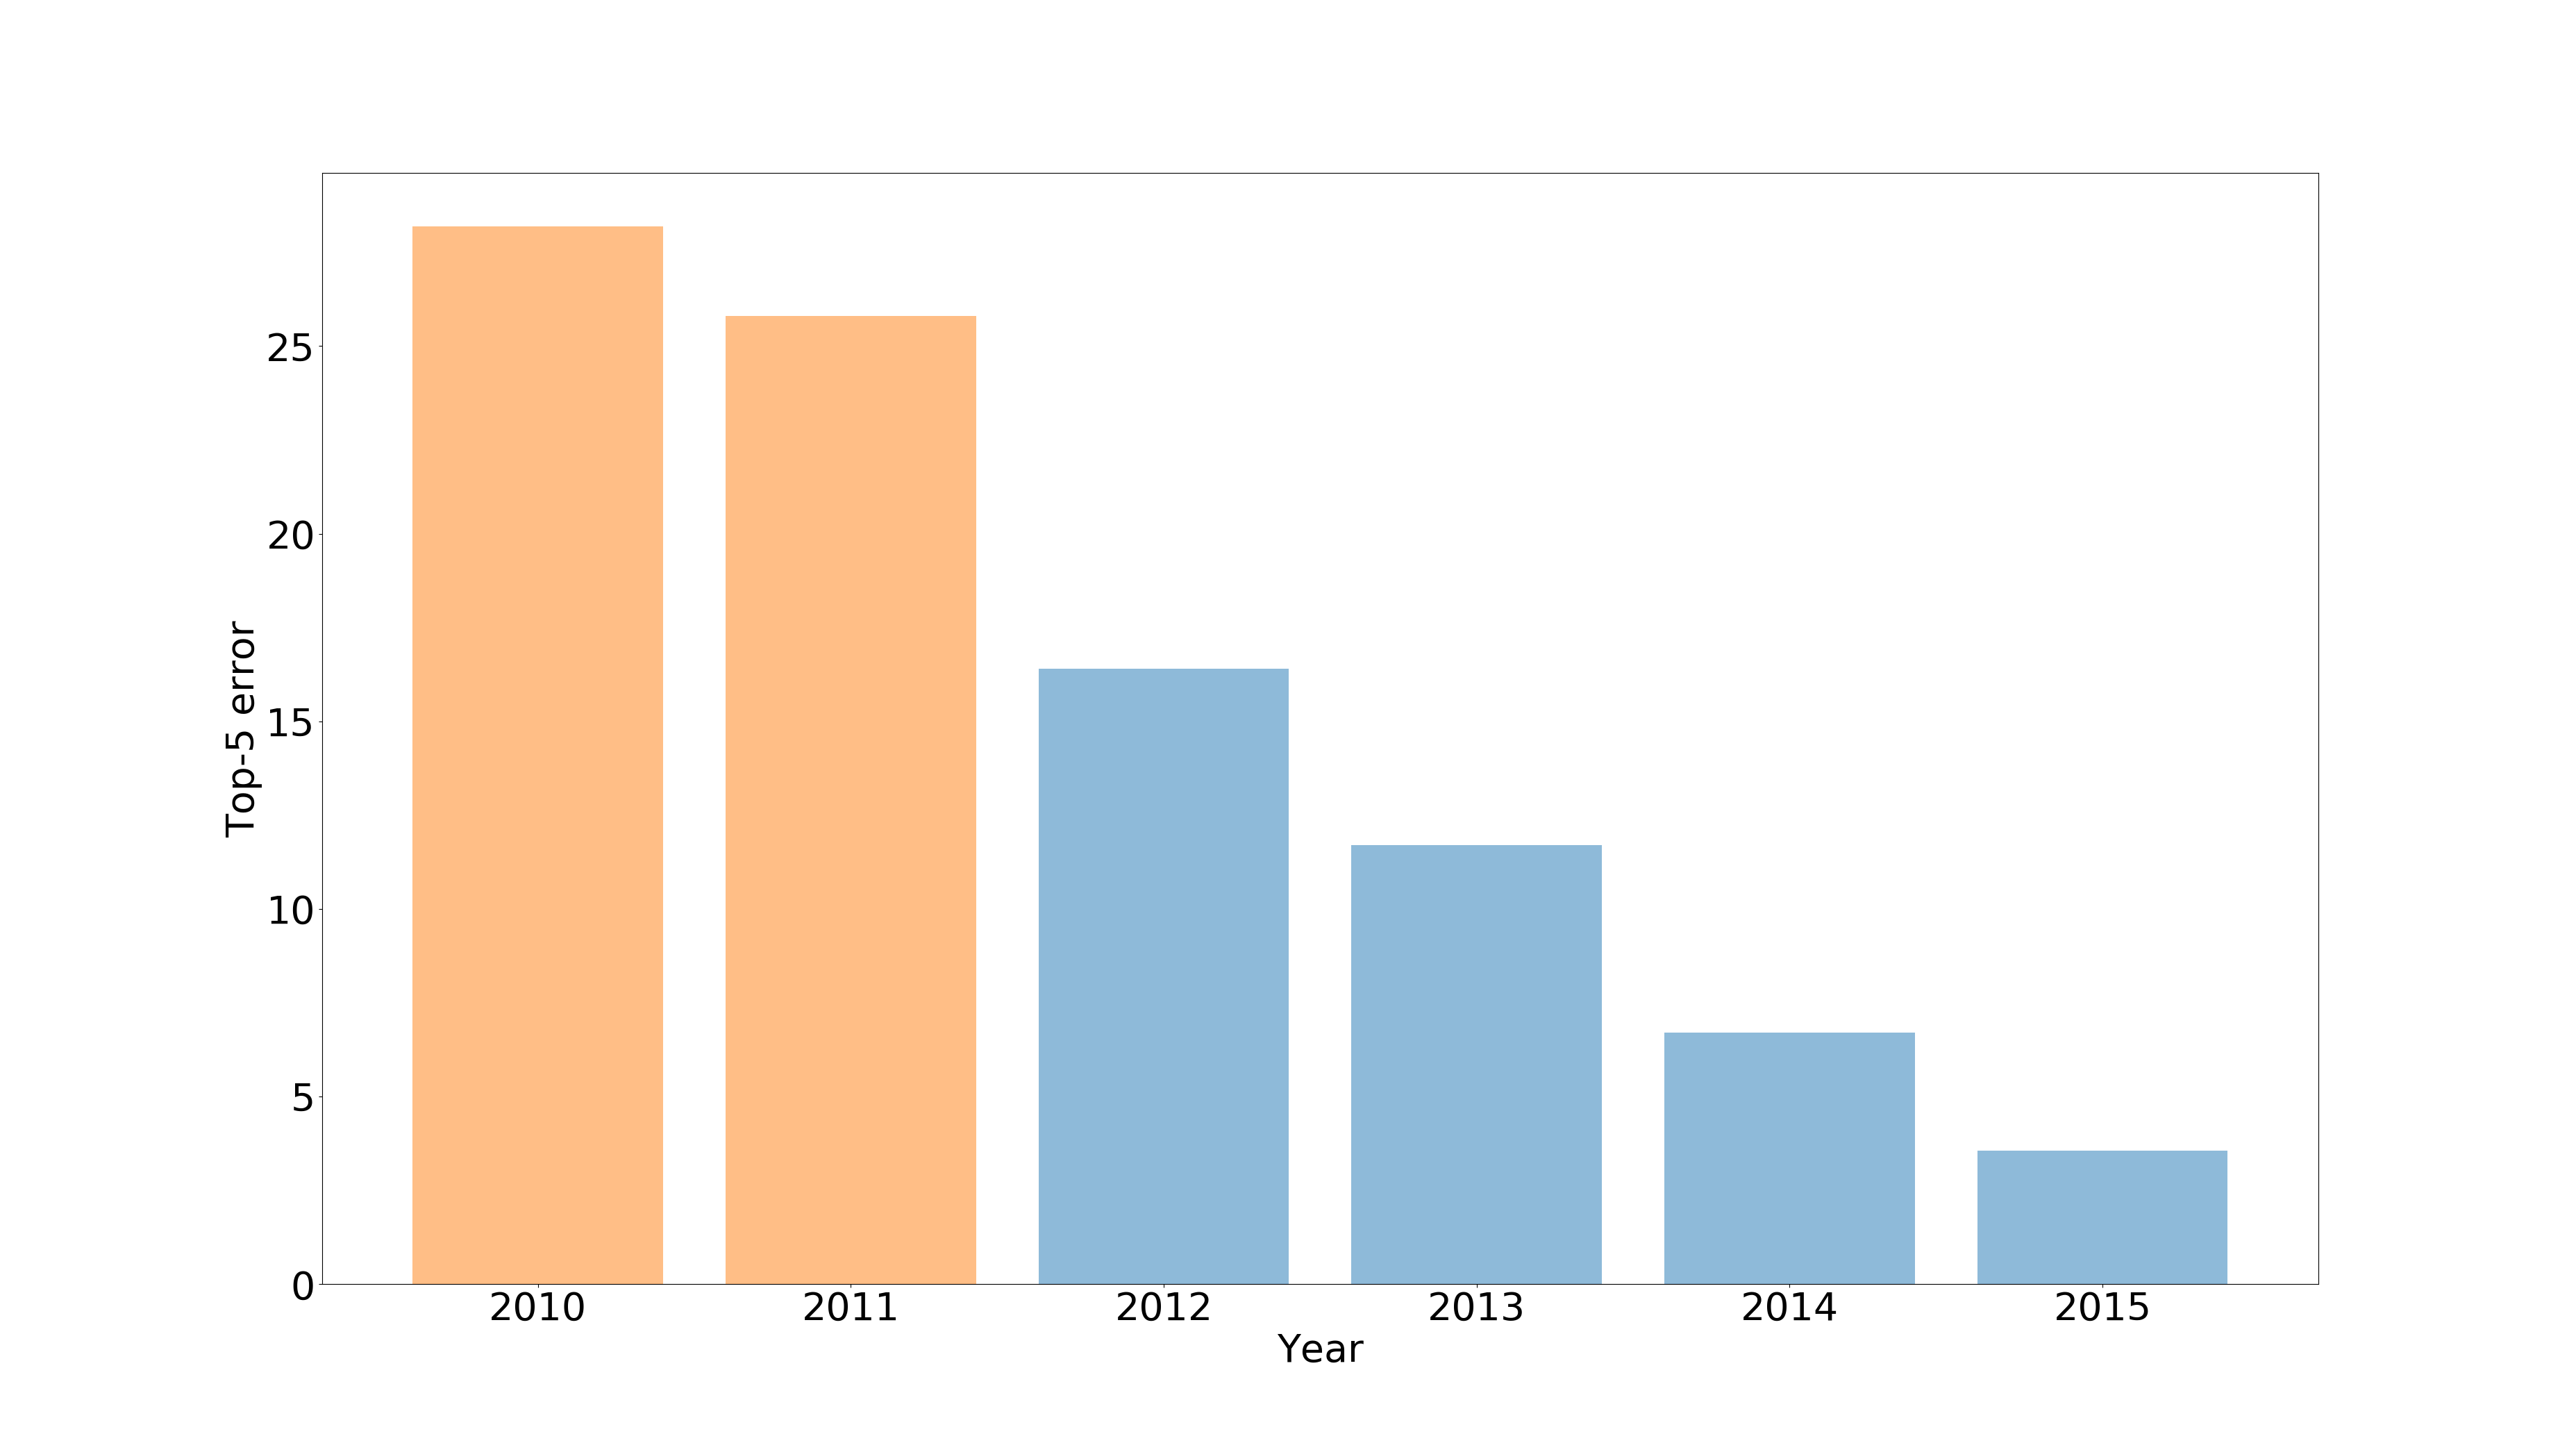
\includegraphics[width=120mm]{./deepLearning/topError.png}

\end{figure}



\end{frame}

\subsection{Objetives}


\begin{frame}{Objetives}


Develop and characterize an algorithm of multiple people tracking, combining:


\hspace{2cm}

\begin{itemize}

\item Neural networks

\item Feature-based tracking

\end{itemize}


\hspace{2cm}

Testing of the component on an international databases, the Multiple object tracking challenge.

\end{frame}


%
%\begin{frame}{Tracking paradigms}
%
%
%\begin{itemize}
%
%
%\item \textbf{Tracking-by-detection}
%
%\item \textbf{Tracking learning and detection}
%
%
%\item \textbf{Siamese based tracking}
%
%
%\item \textbf{Tracking as regression}
%
%
%\item \textbf{Tracking with Recurrent Neural Networks} 
%
%\end{itemize}
%\end{frame}


\section{Software implementation}

\begin{frame}{System Overview: Diagram}

\begin{figure}[htbp]
\centering
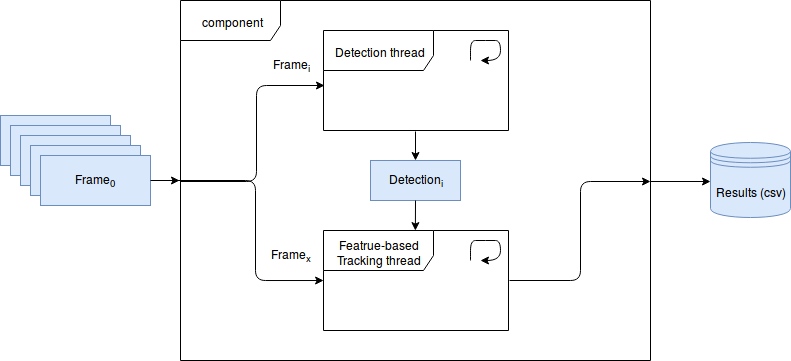
\includegraphics[width=90mm]{./algoritme/bloque2.png}

\end{figure}



\end{frame}


\begin{frame}{System Overview: Temporal diagram}

\begin{figure}[htbp]
\centering
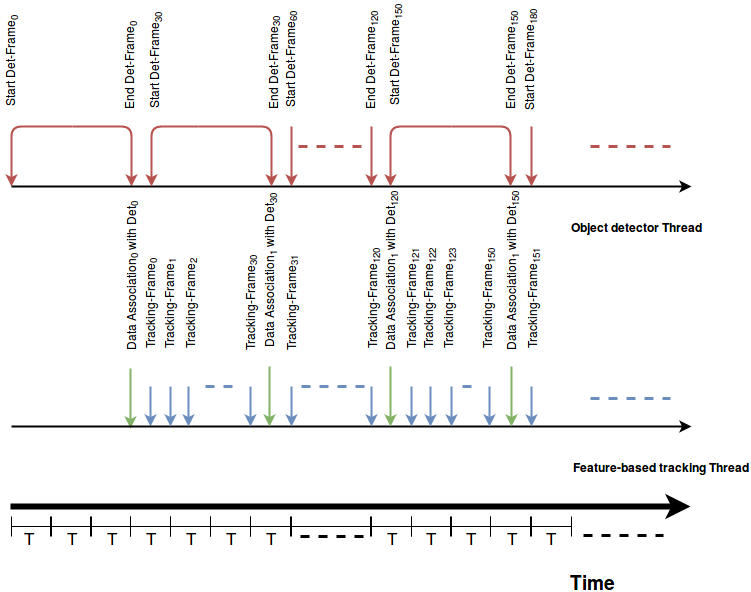
\includegraphics[width=90mm]{./algoritme/timeFInas3.png}

\end{figure}



\end{frame}

\subsection{Object detection thread}

\begin{frame}{Object detector thread: Overview}



\begin{figure}[htbp]
\centering
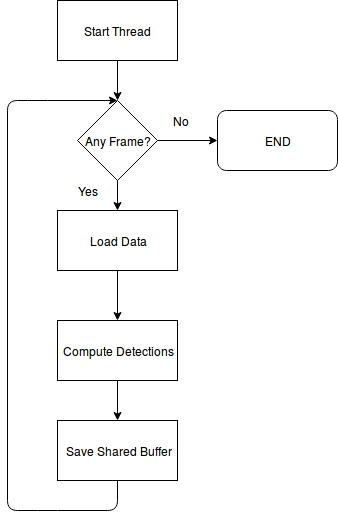
\includegraphics[width=40mm]{./algoritme/detetc.png}

\end{figure}






\end{frame}


%
%\begin{frame}{Object detectors with deep learning}
%
%
%
%\begin{itemize}
%
%
%\item Faster Region Proposal Networks [Faster-RCNN]
%\item Single Shot Multibox Detector [SSD]
%\item Region-based Fully Convolutional Networks [RFCN]
%
%\end{itemize}
%
%
%
%\end{frame}



\begin{frame}{Single Shot Multibox Detector [SSD] I}



\begin{figure}[htbp]
\centering
\begin{tabular}{cc}

\subfloat[Input image. ]{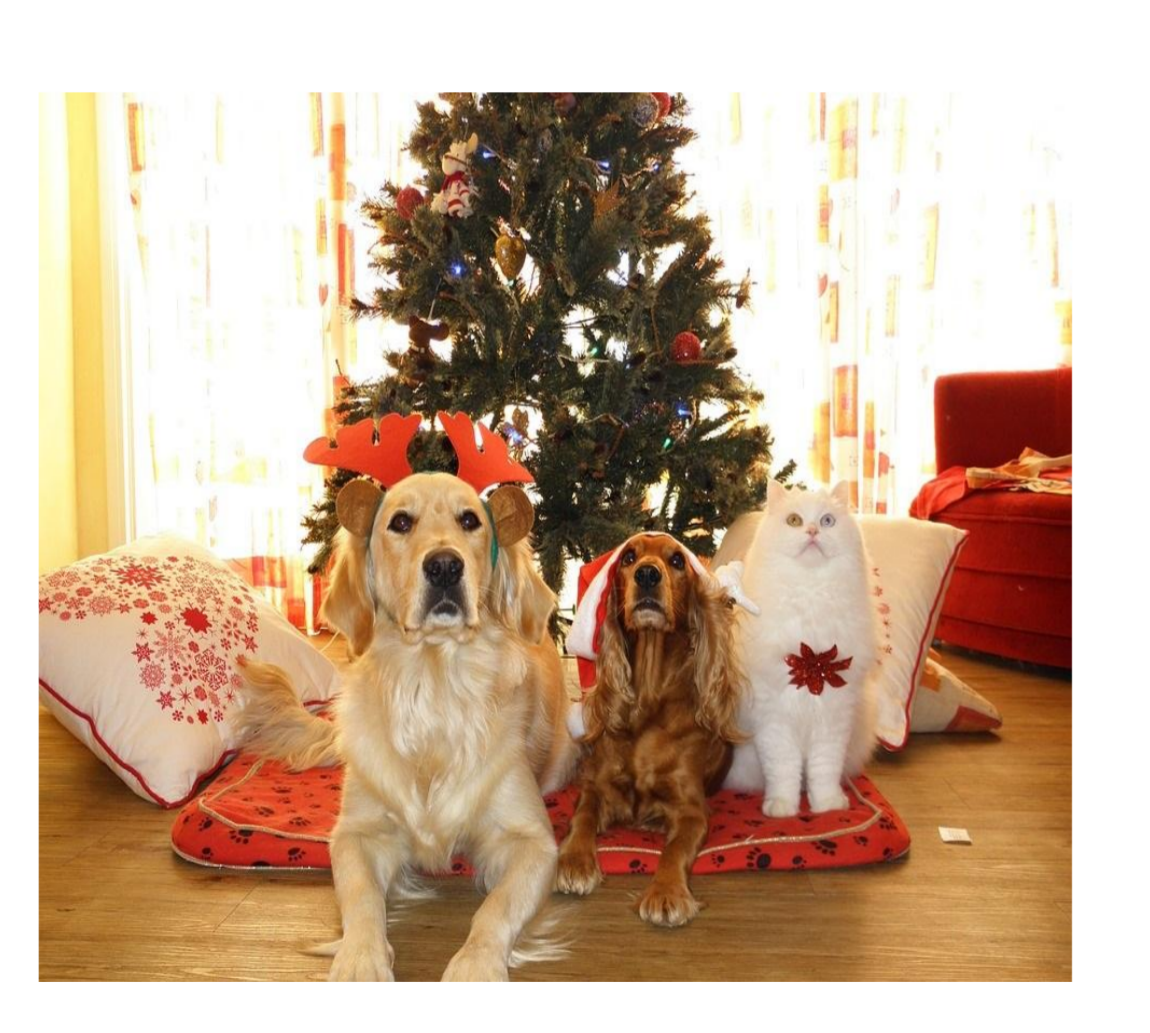
\includegraphics[width=45mm]{./objectdetector/retall1.png}}&
\subfloat[Divided image.]{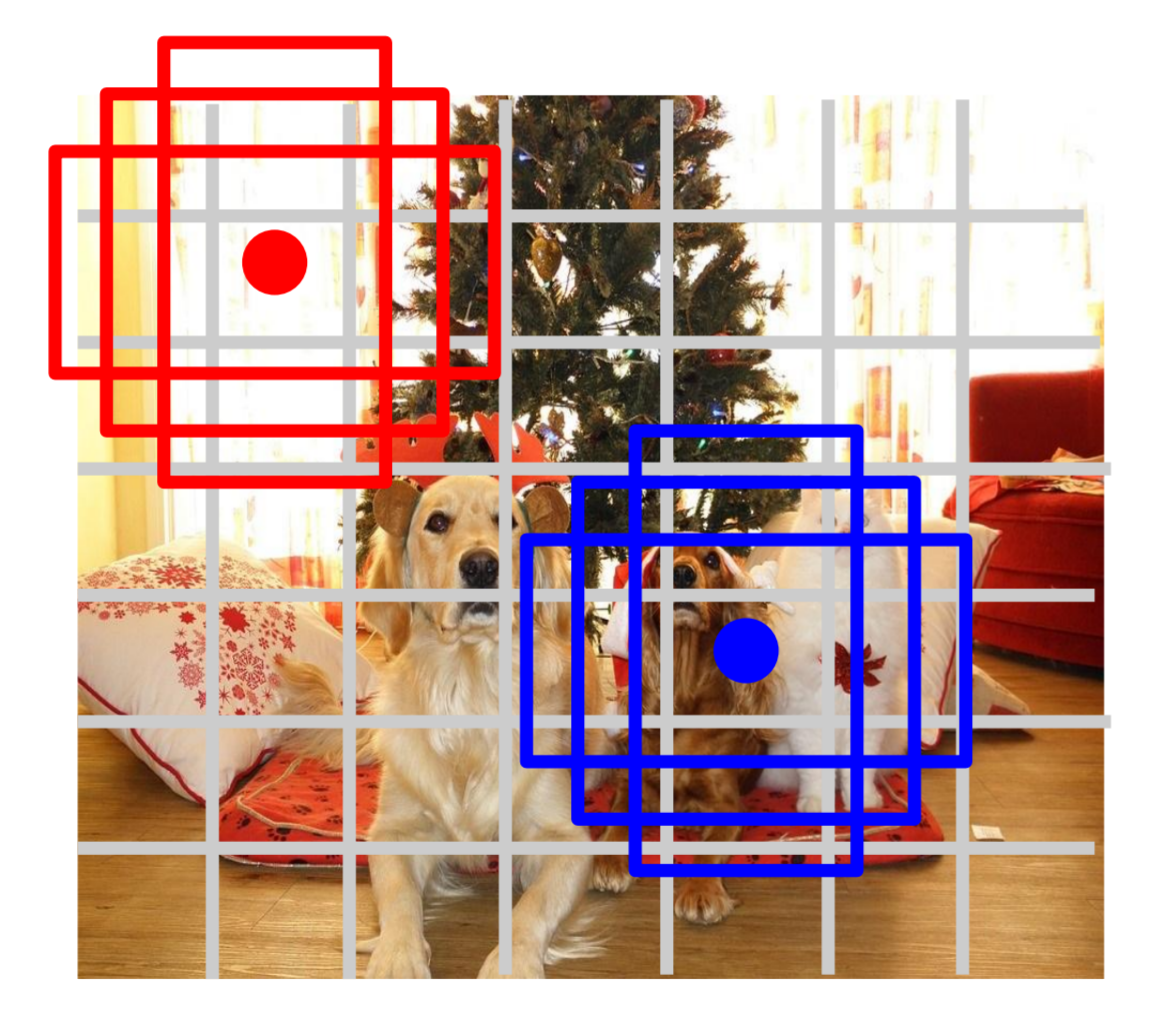
\includegraphics[width=45mm]{./objectdetector/retall2.png}}\\



\end{tabular}
%\caption{Imatges MRI amb tumor.} \label{pseudo}
\end{figure}


\end{frame}



\begin{frame}{Single Shot Multibox Detector [SSD] II}


\begin{figure}[htbp]
\centering
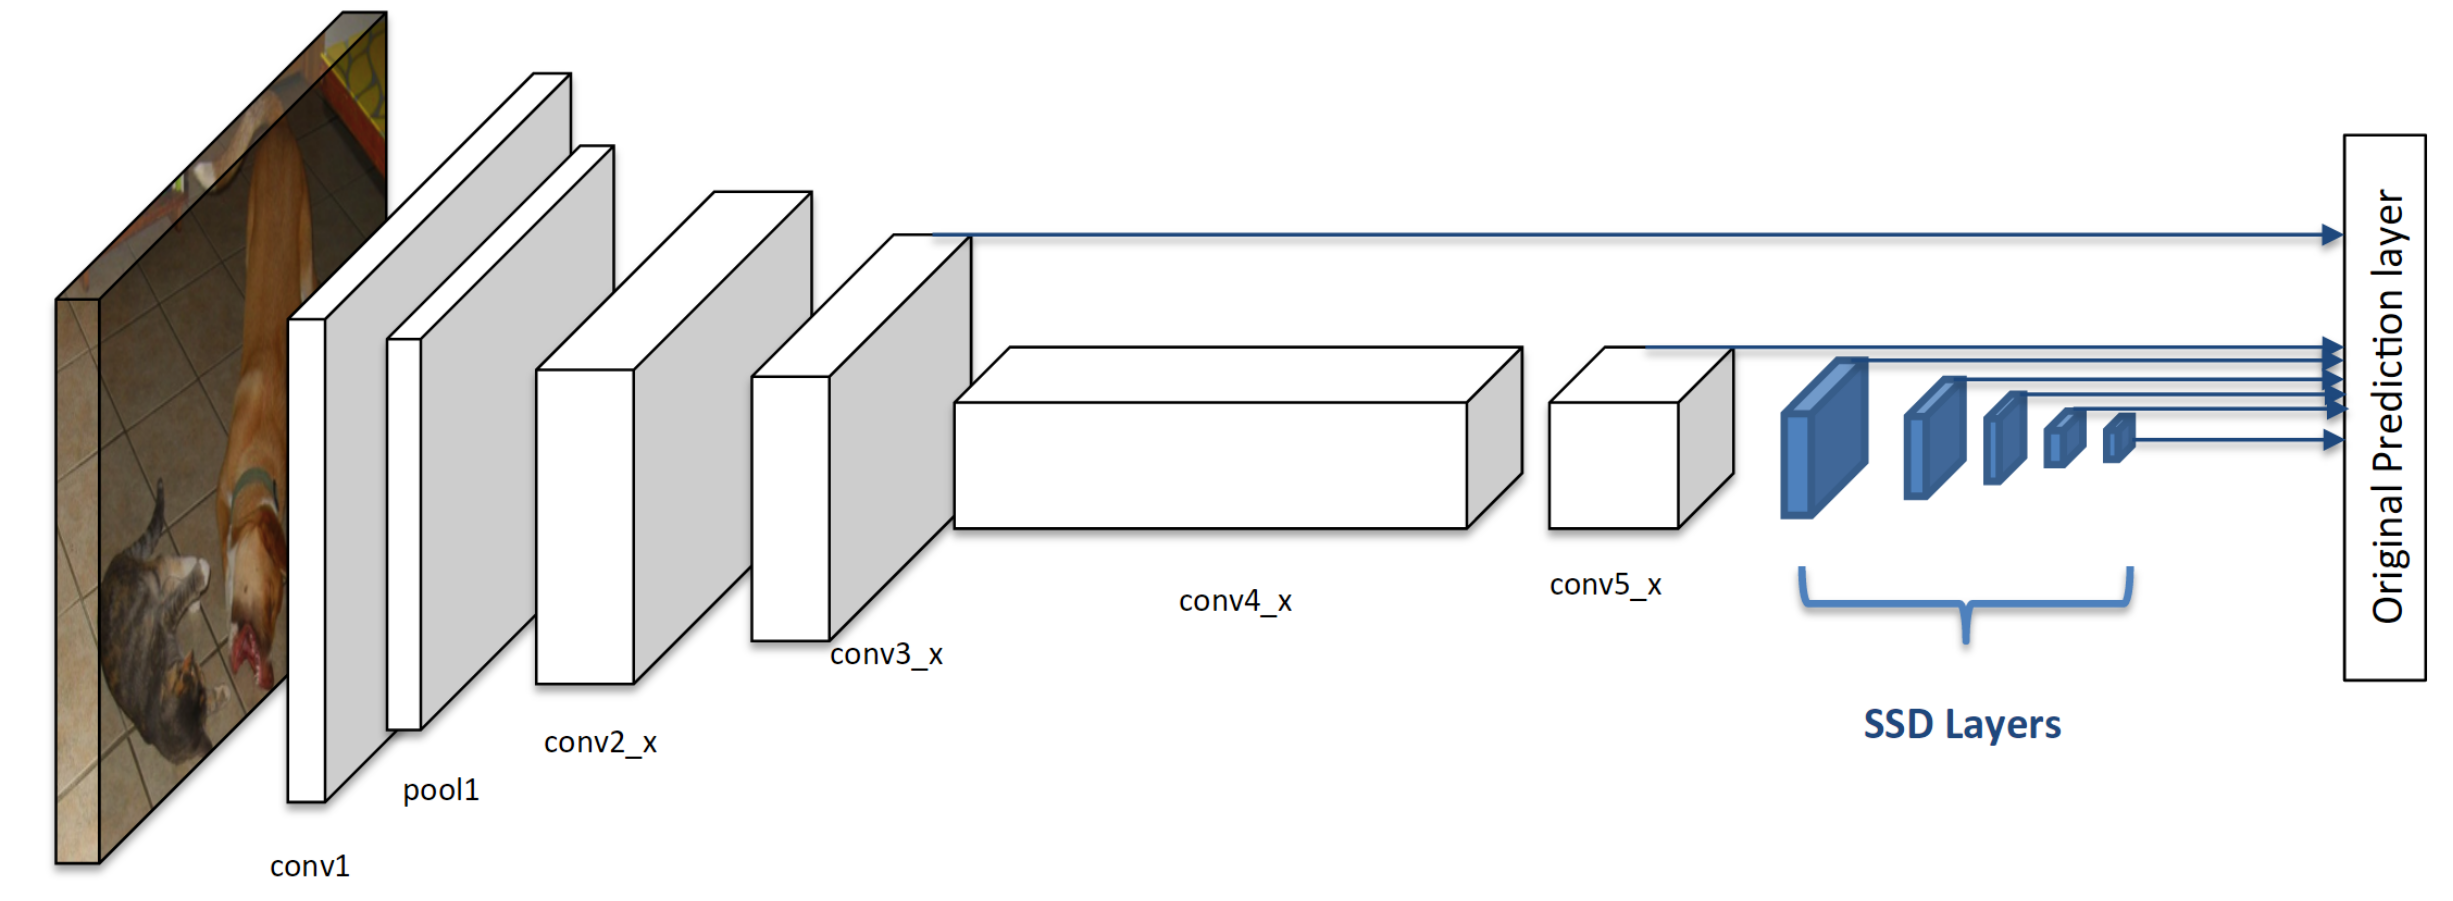
\includegraphics[width=100mm]{./objectdetector/ssdArchitecture2.png}

\end{figure}






\end{frame}




\begin{frame}{Result Object detector thread}


\begin{figure}[htbp]
\centering
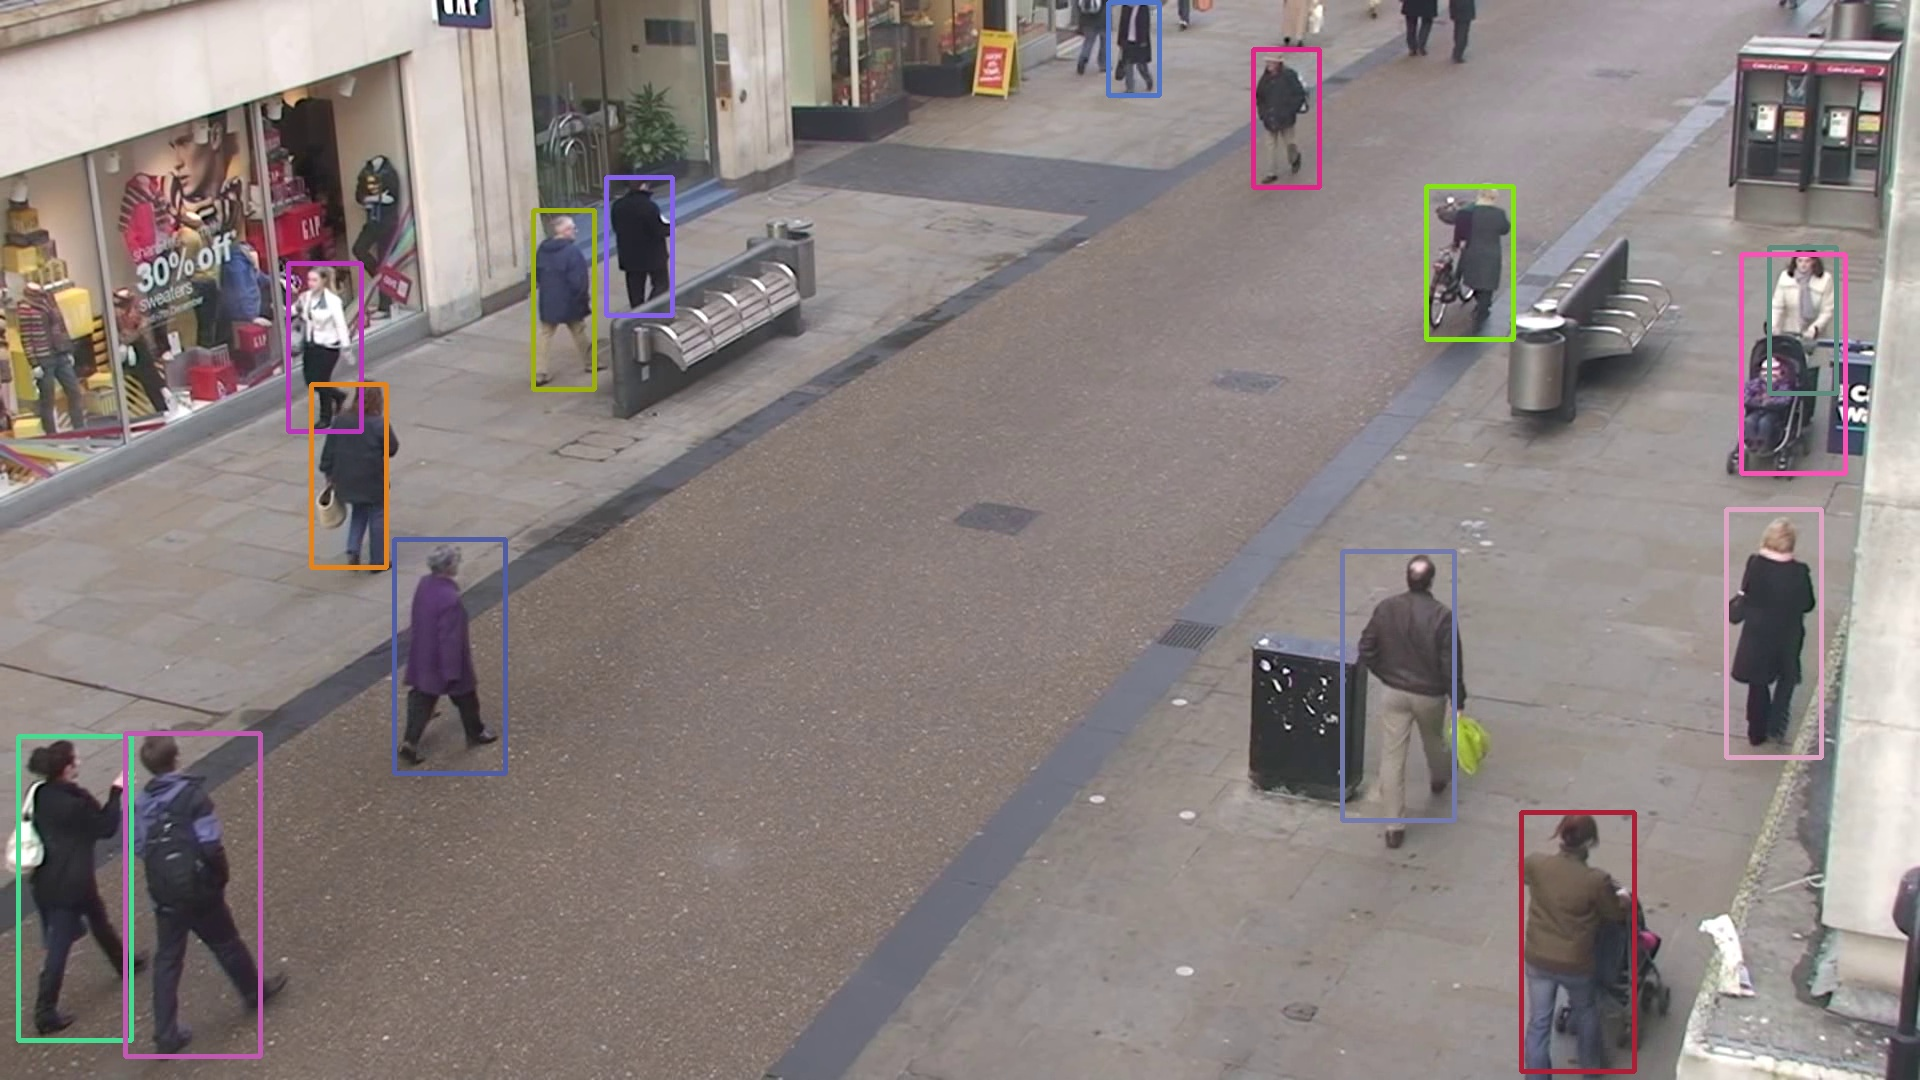
\includegraphics[width=120mm]{./objectdetector/deteccions.jpg}

\end{figure}


\end{frame}



%-----------------------------------------------------------------------------
\subsection{Feature-based tracking thread}
\begin{frame}{Feature-based tracking thread: Overview}



\begin{figure}[htbp]
\centering
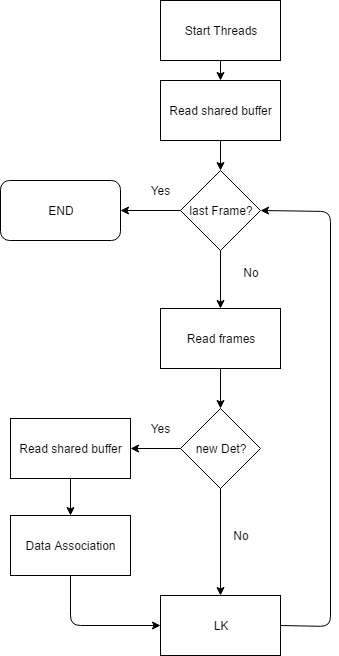
\includegraphics[width=37mm]{./algoritme/arc.png}

\end{figure}


\end{frame}


\begin{frame}{Feature-based tracking overview}



\begin{figure}[htbp]
\centering
\begin{tabular}{cccc}

\subfloat[Detection. ]{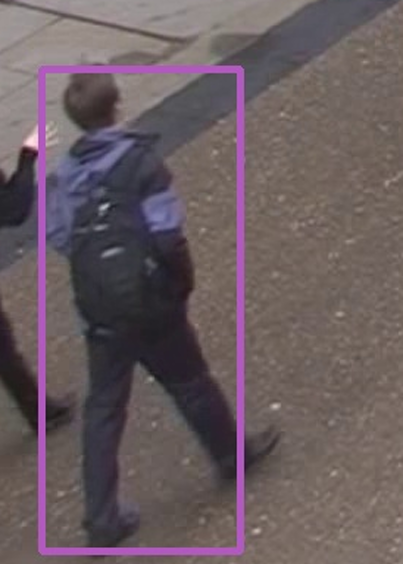
\includegraphics[width=25mm]{./tracker/bounding1.png}}&
\subfloat[Points.]{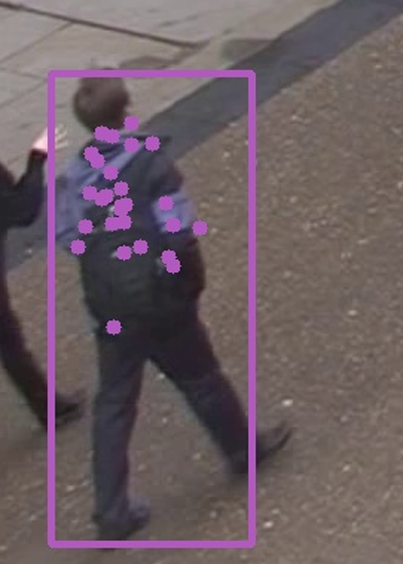
\includegraphics[width=25mm]{./tracker/ppints1.png}}&
\subfloat[Matching.]{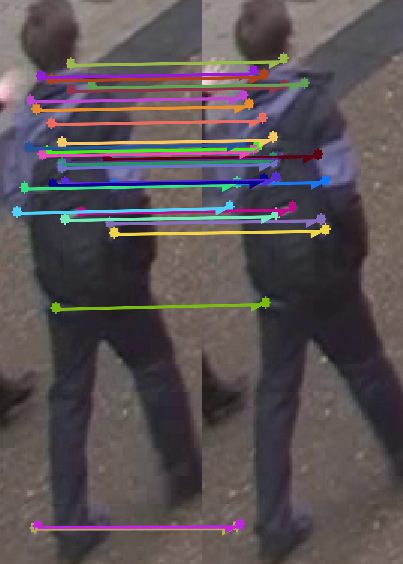
\includegraphics[width=25mm]{./tracker/matching3b.png}}&
\subfloat[Displacement.]{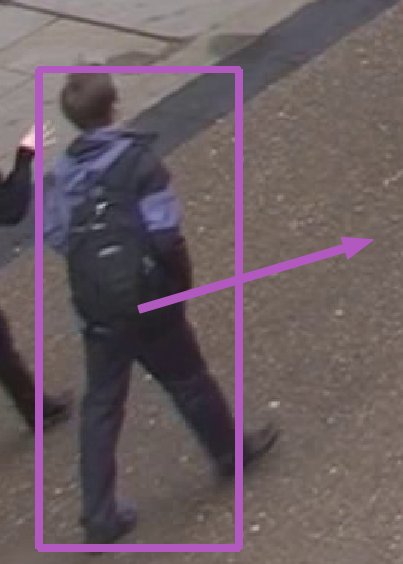
\includegraphics[width=25mm]{./tracker/arrow1.png}}\\



\end{tabular}
%\caption{Imatges MRI amb tumor.} \label{pseudo}
\end{figure}


\end{frame}






%\begin{frame}{Feature extraction}
%
%
%\begin{figure}[htbp]
%\centering
%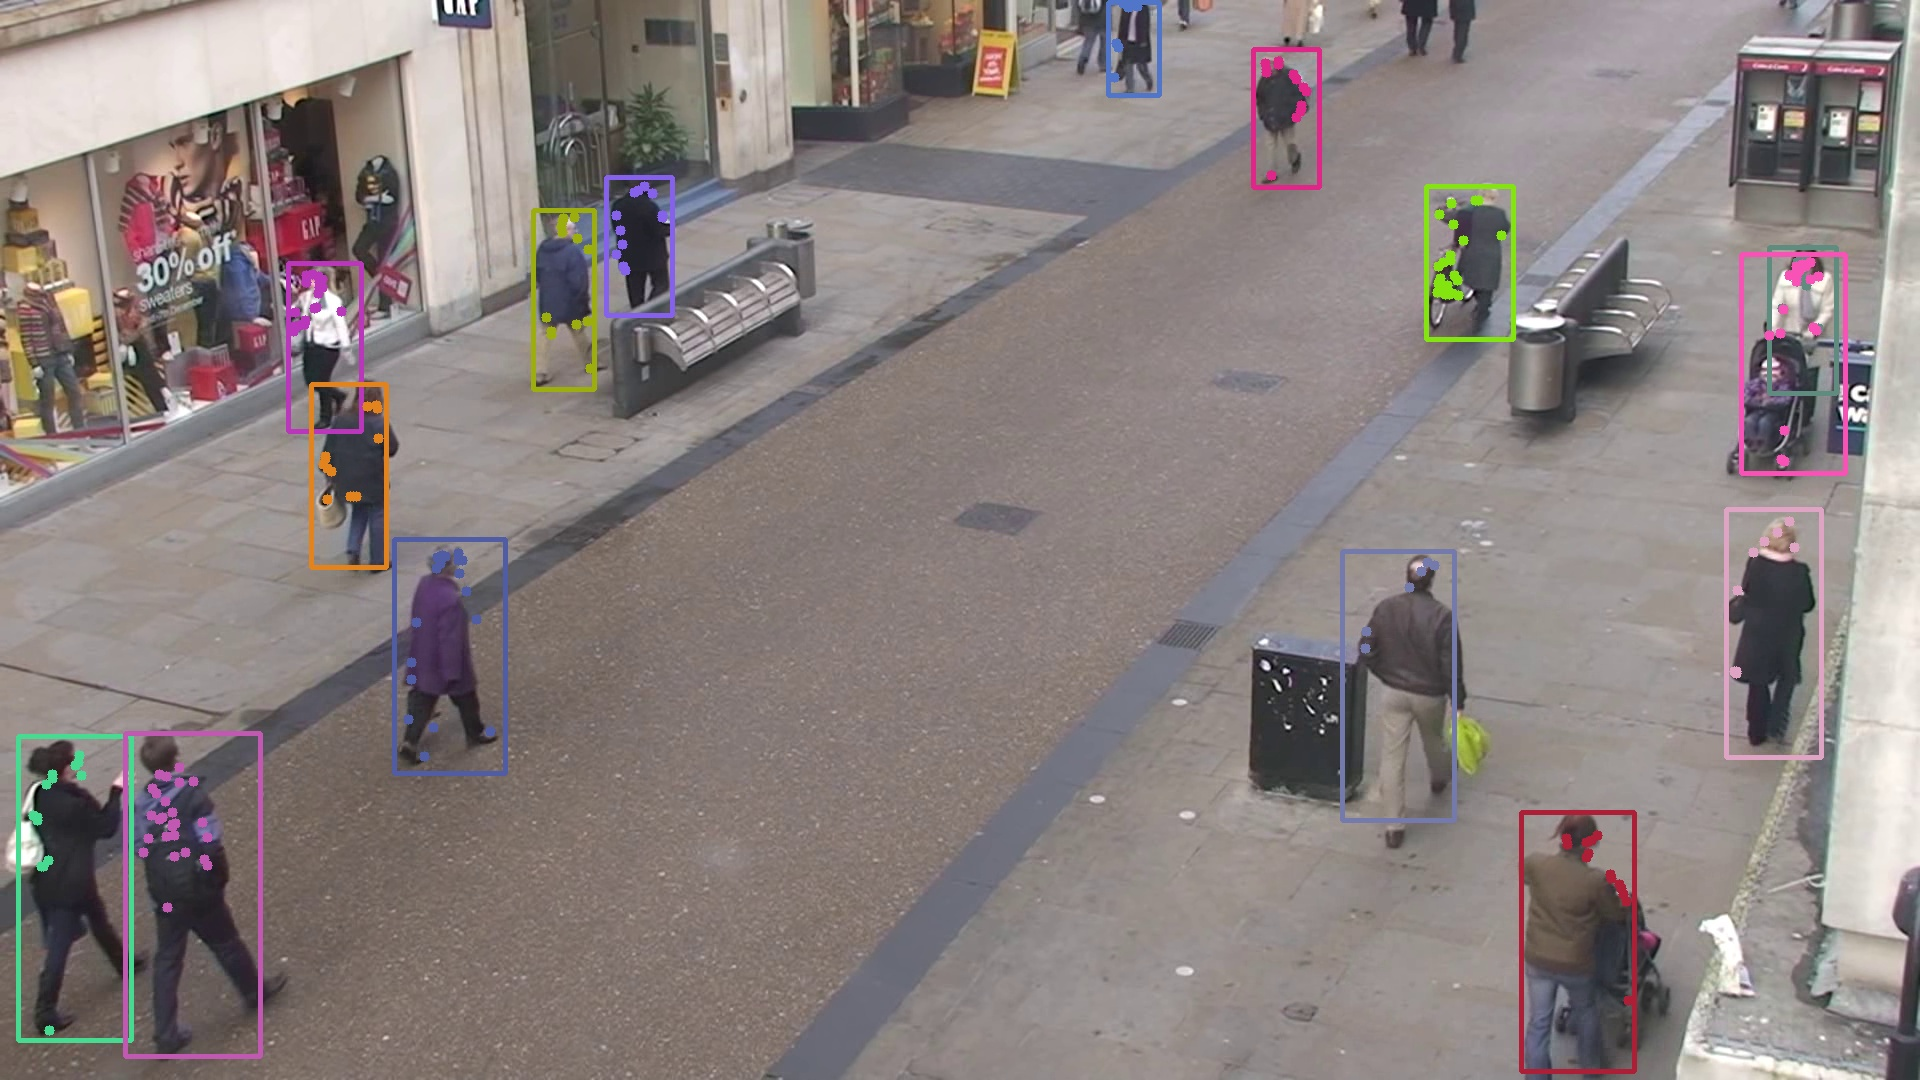
\includegraphics[width=120mm]{./tracker/pounts.jpg}
%
%\end{figure}
%
%
%
%
%\end{frame}


%\begin{frame}{Matching blobs}
%
%
%\begin{figure}[htbp]
%\centering
%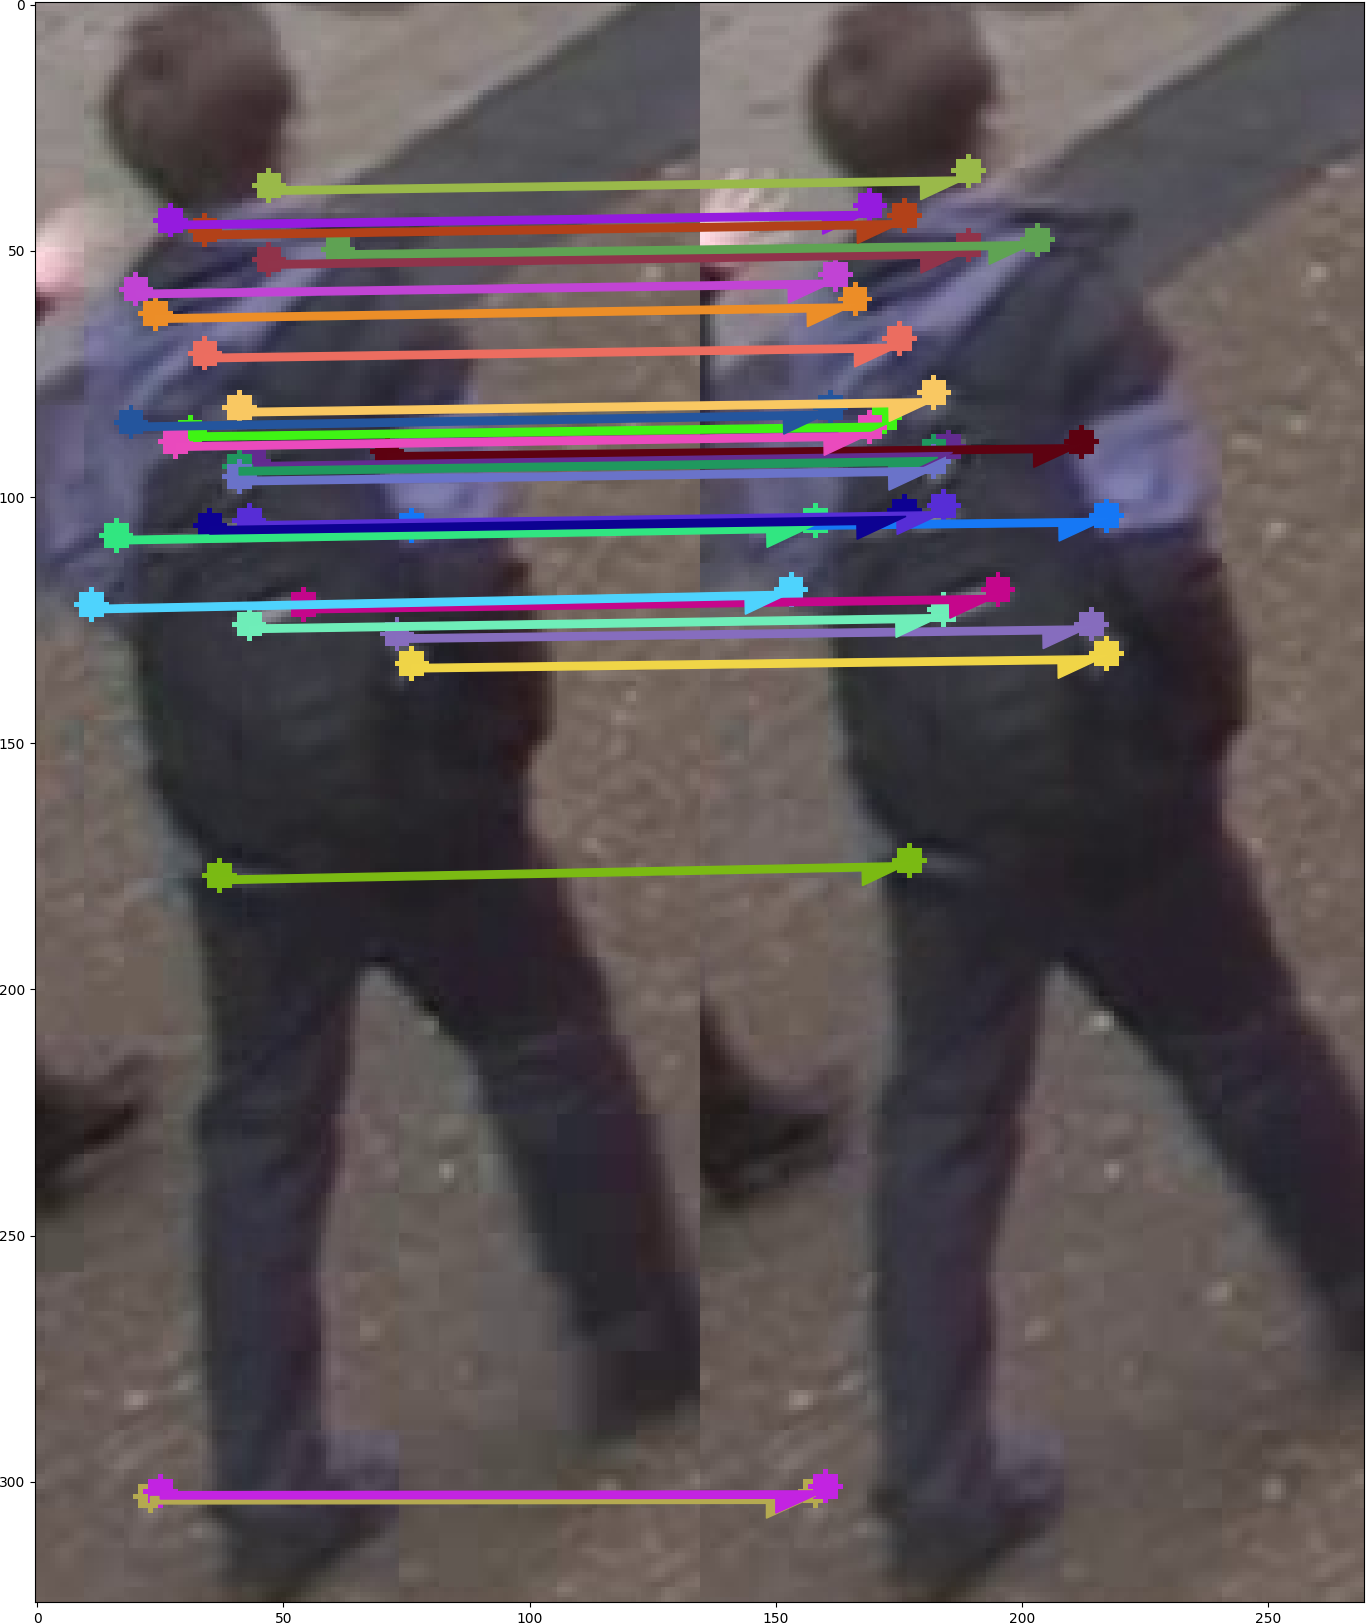
\includegraphics[width=60mm]{./tracker/matching.png}
%
%\end{figure}
%
%
%
%
%\end{frame}

\begin{frame}{Blobs}


\begin{figure}[htbp]
\centering
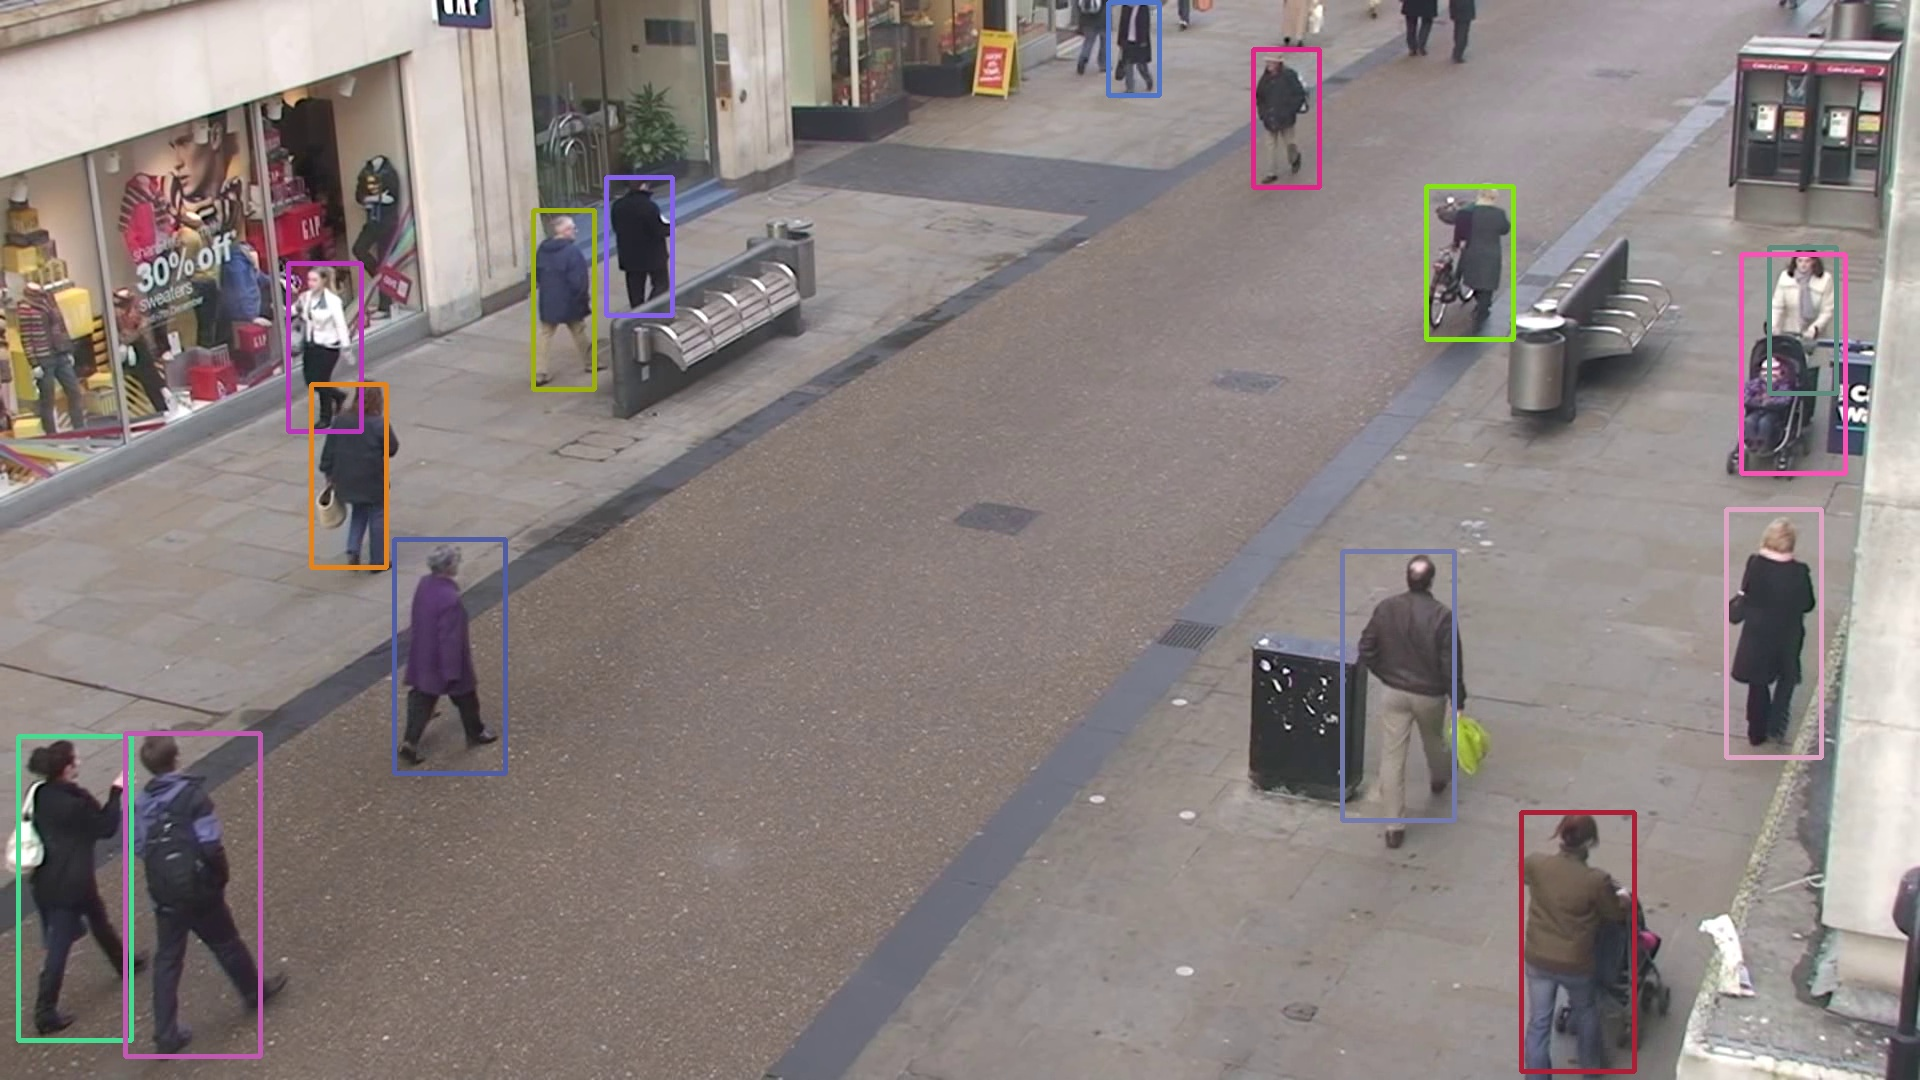
\includegraphics[width=120mm]{./objectdetector/deteccions.jpg}

\end{figure}


\end{frame}



\begin{frame}{Displacement}


\begin{figure}[htbp]
\centering
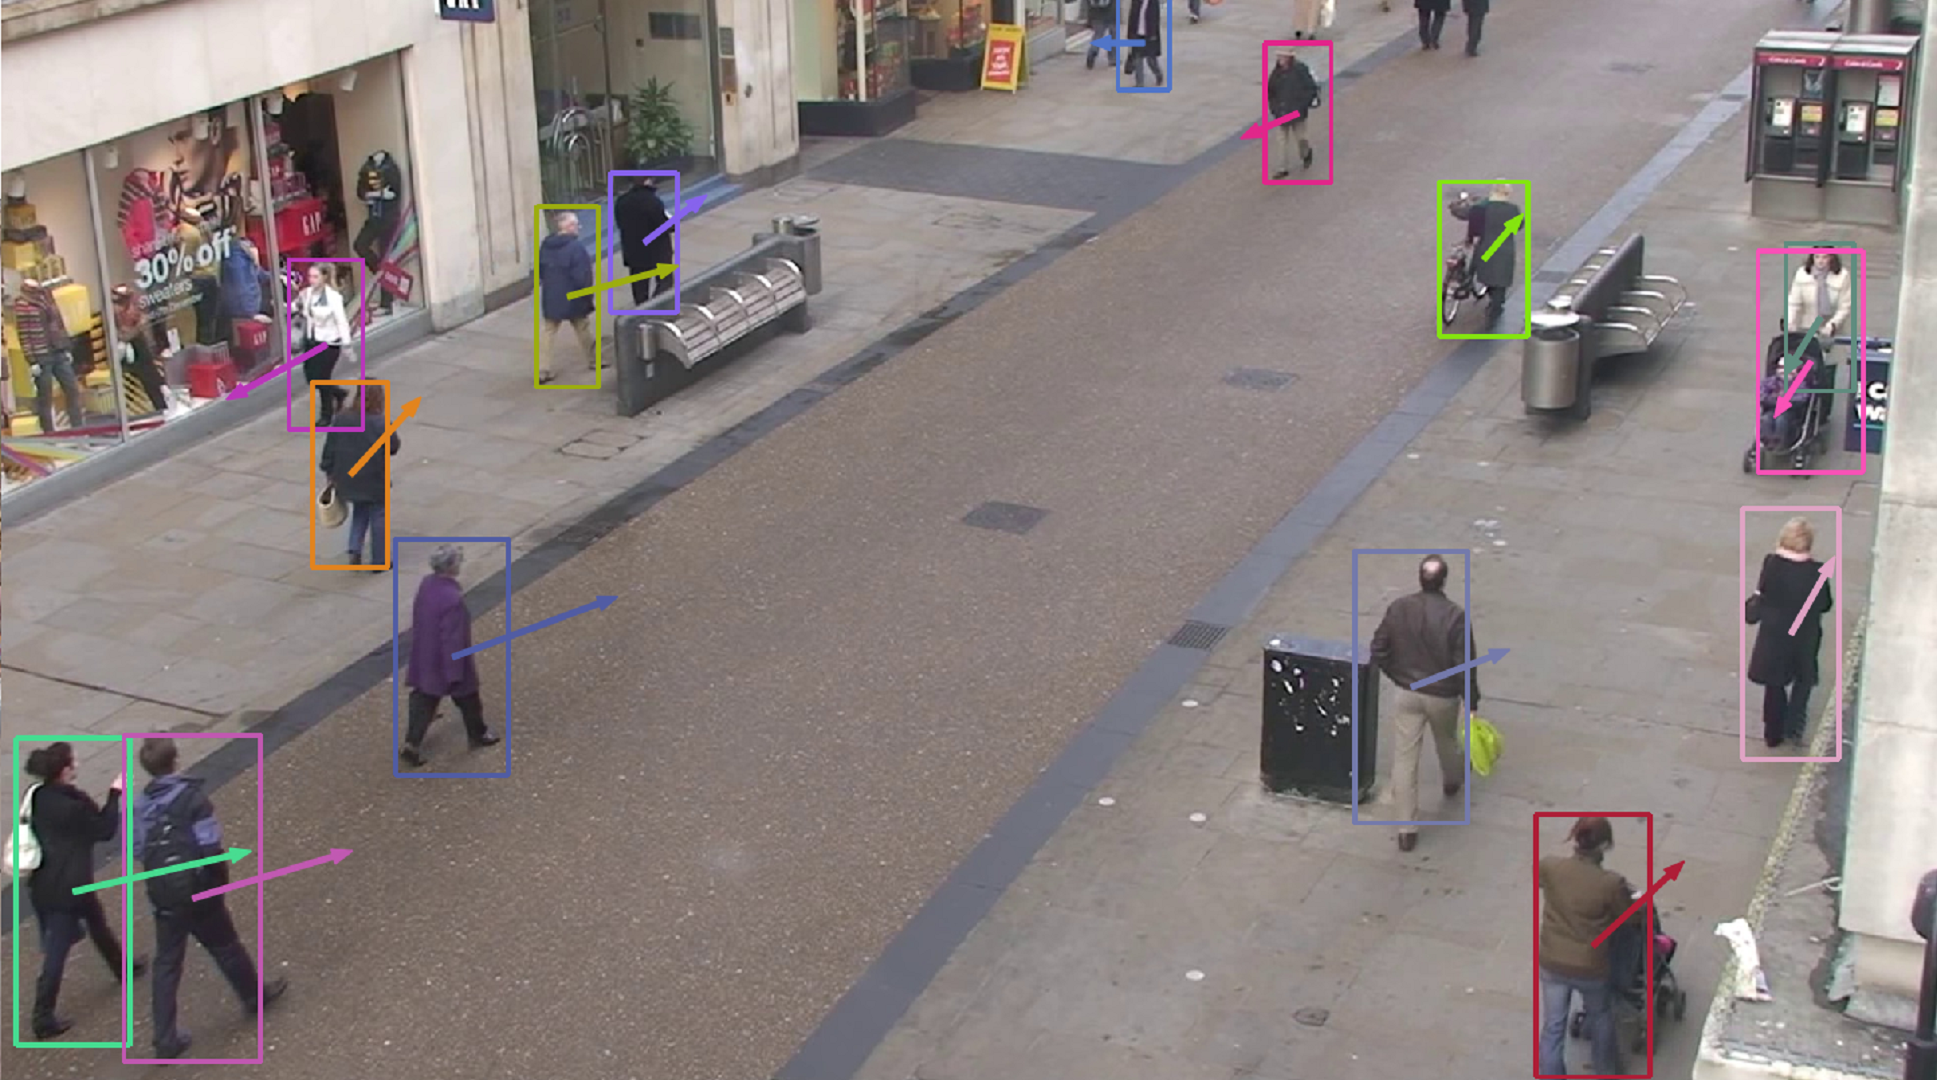
\includegraphics[width=120mm]{./tracker/alcover2.png}

\end{figure}




\end{frame}


\begin{frame}{Upload estimation}


\begin{figure}[htbp]
\centering
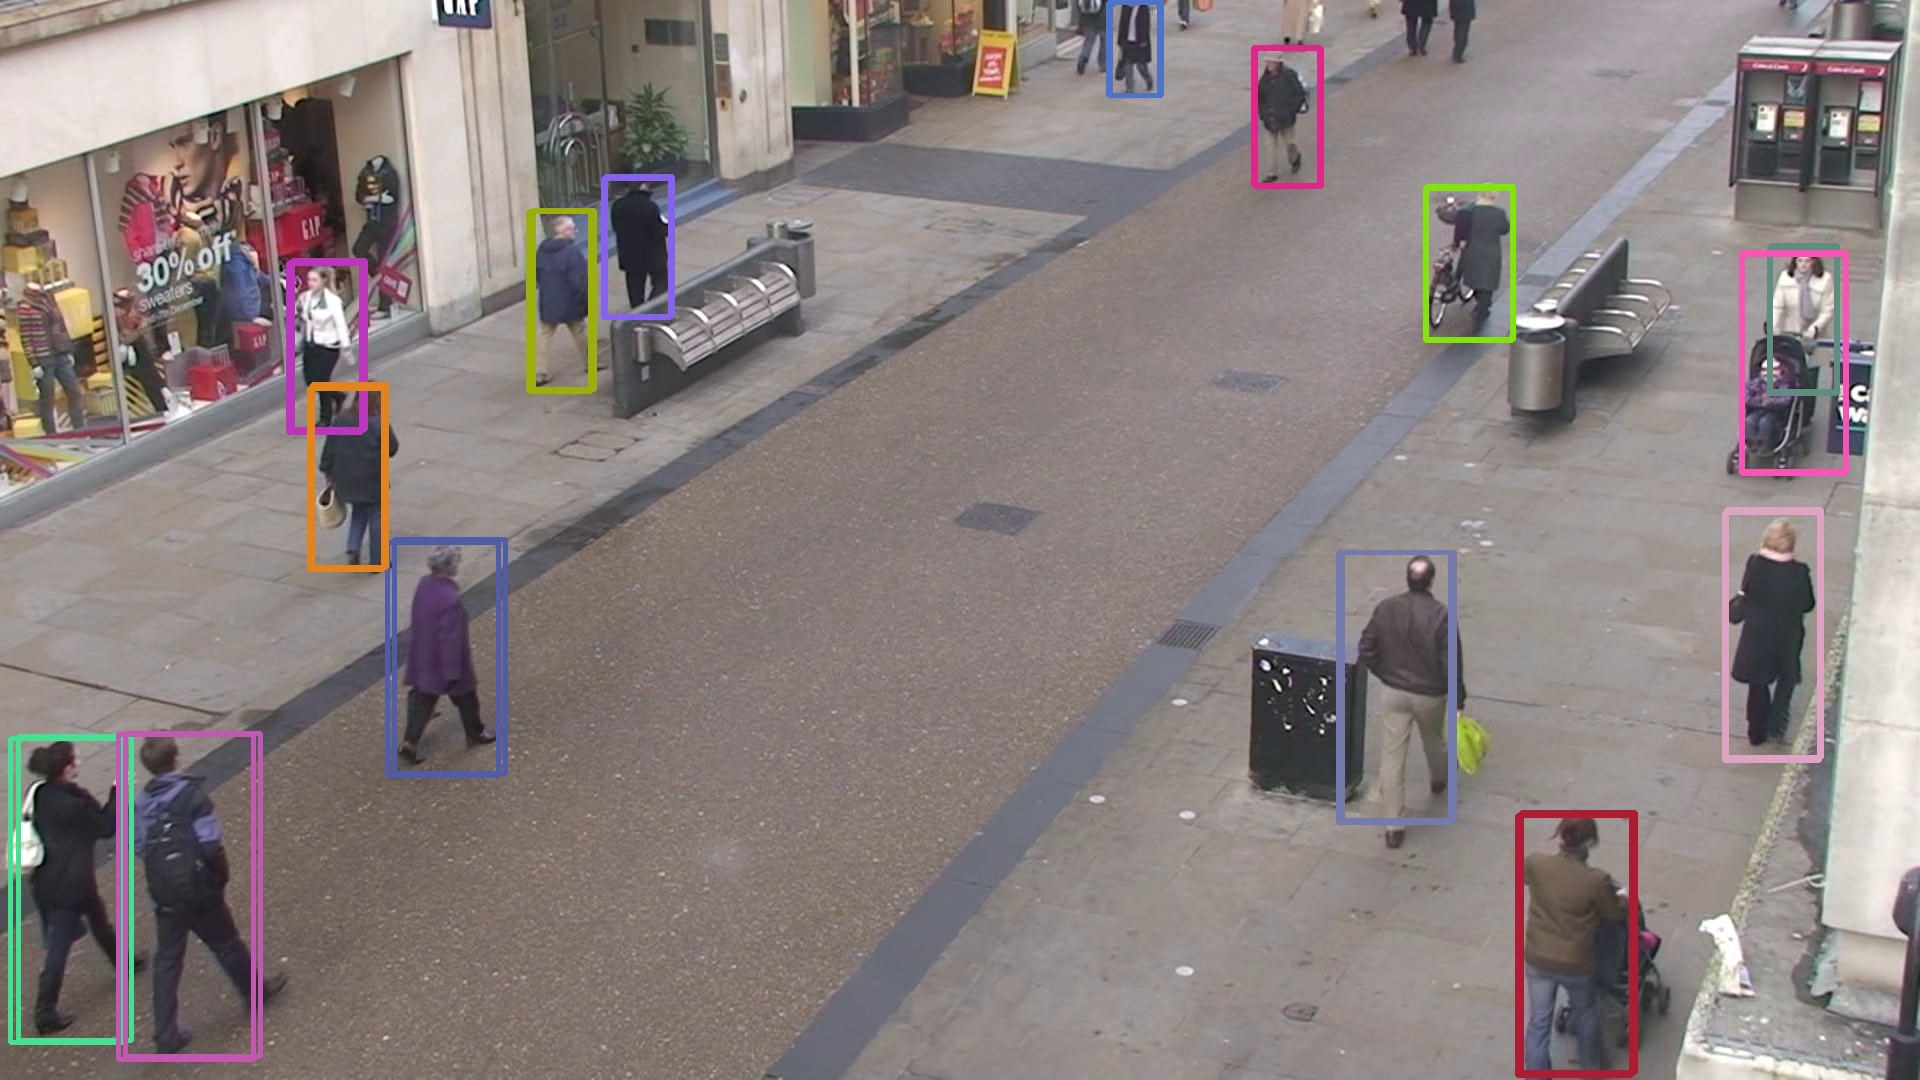
\includegraphics[width=120mm]{./tracker/deteccionsBLOB.jpg}

\end{figure}




\end{frame}


\begin{frame}{Tracking failure}

\begin{figure}[htbp]
\centering
\begin{tabular}{ccc}
\subfloat[Trajectory]{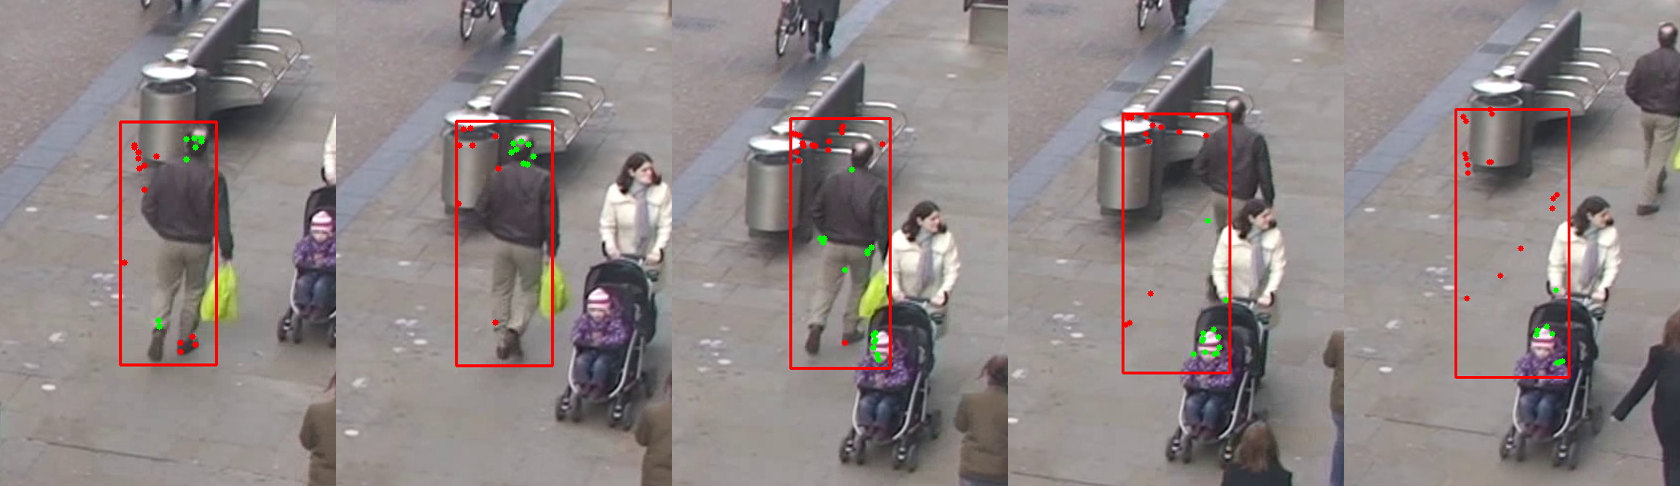
\includegraphics[width=80mm]{velocidadas/mateuPont.png}}\\
\pause
\subfloat[Plots]{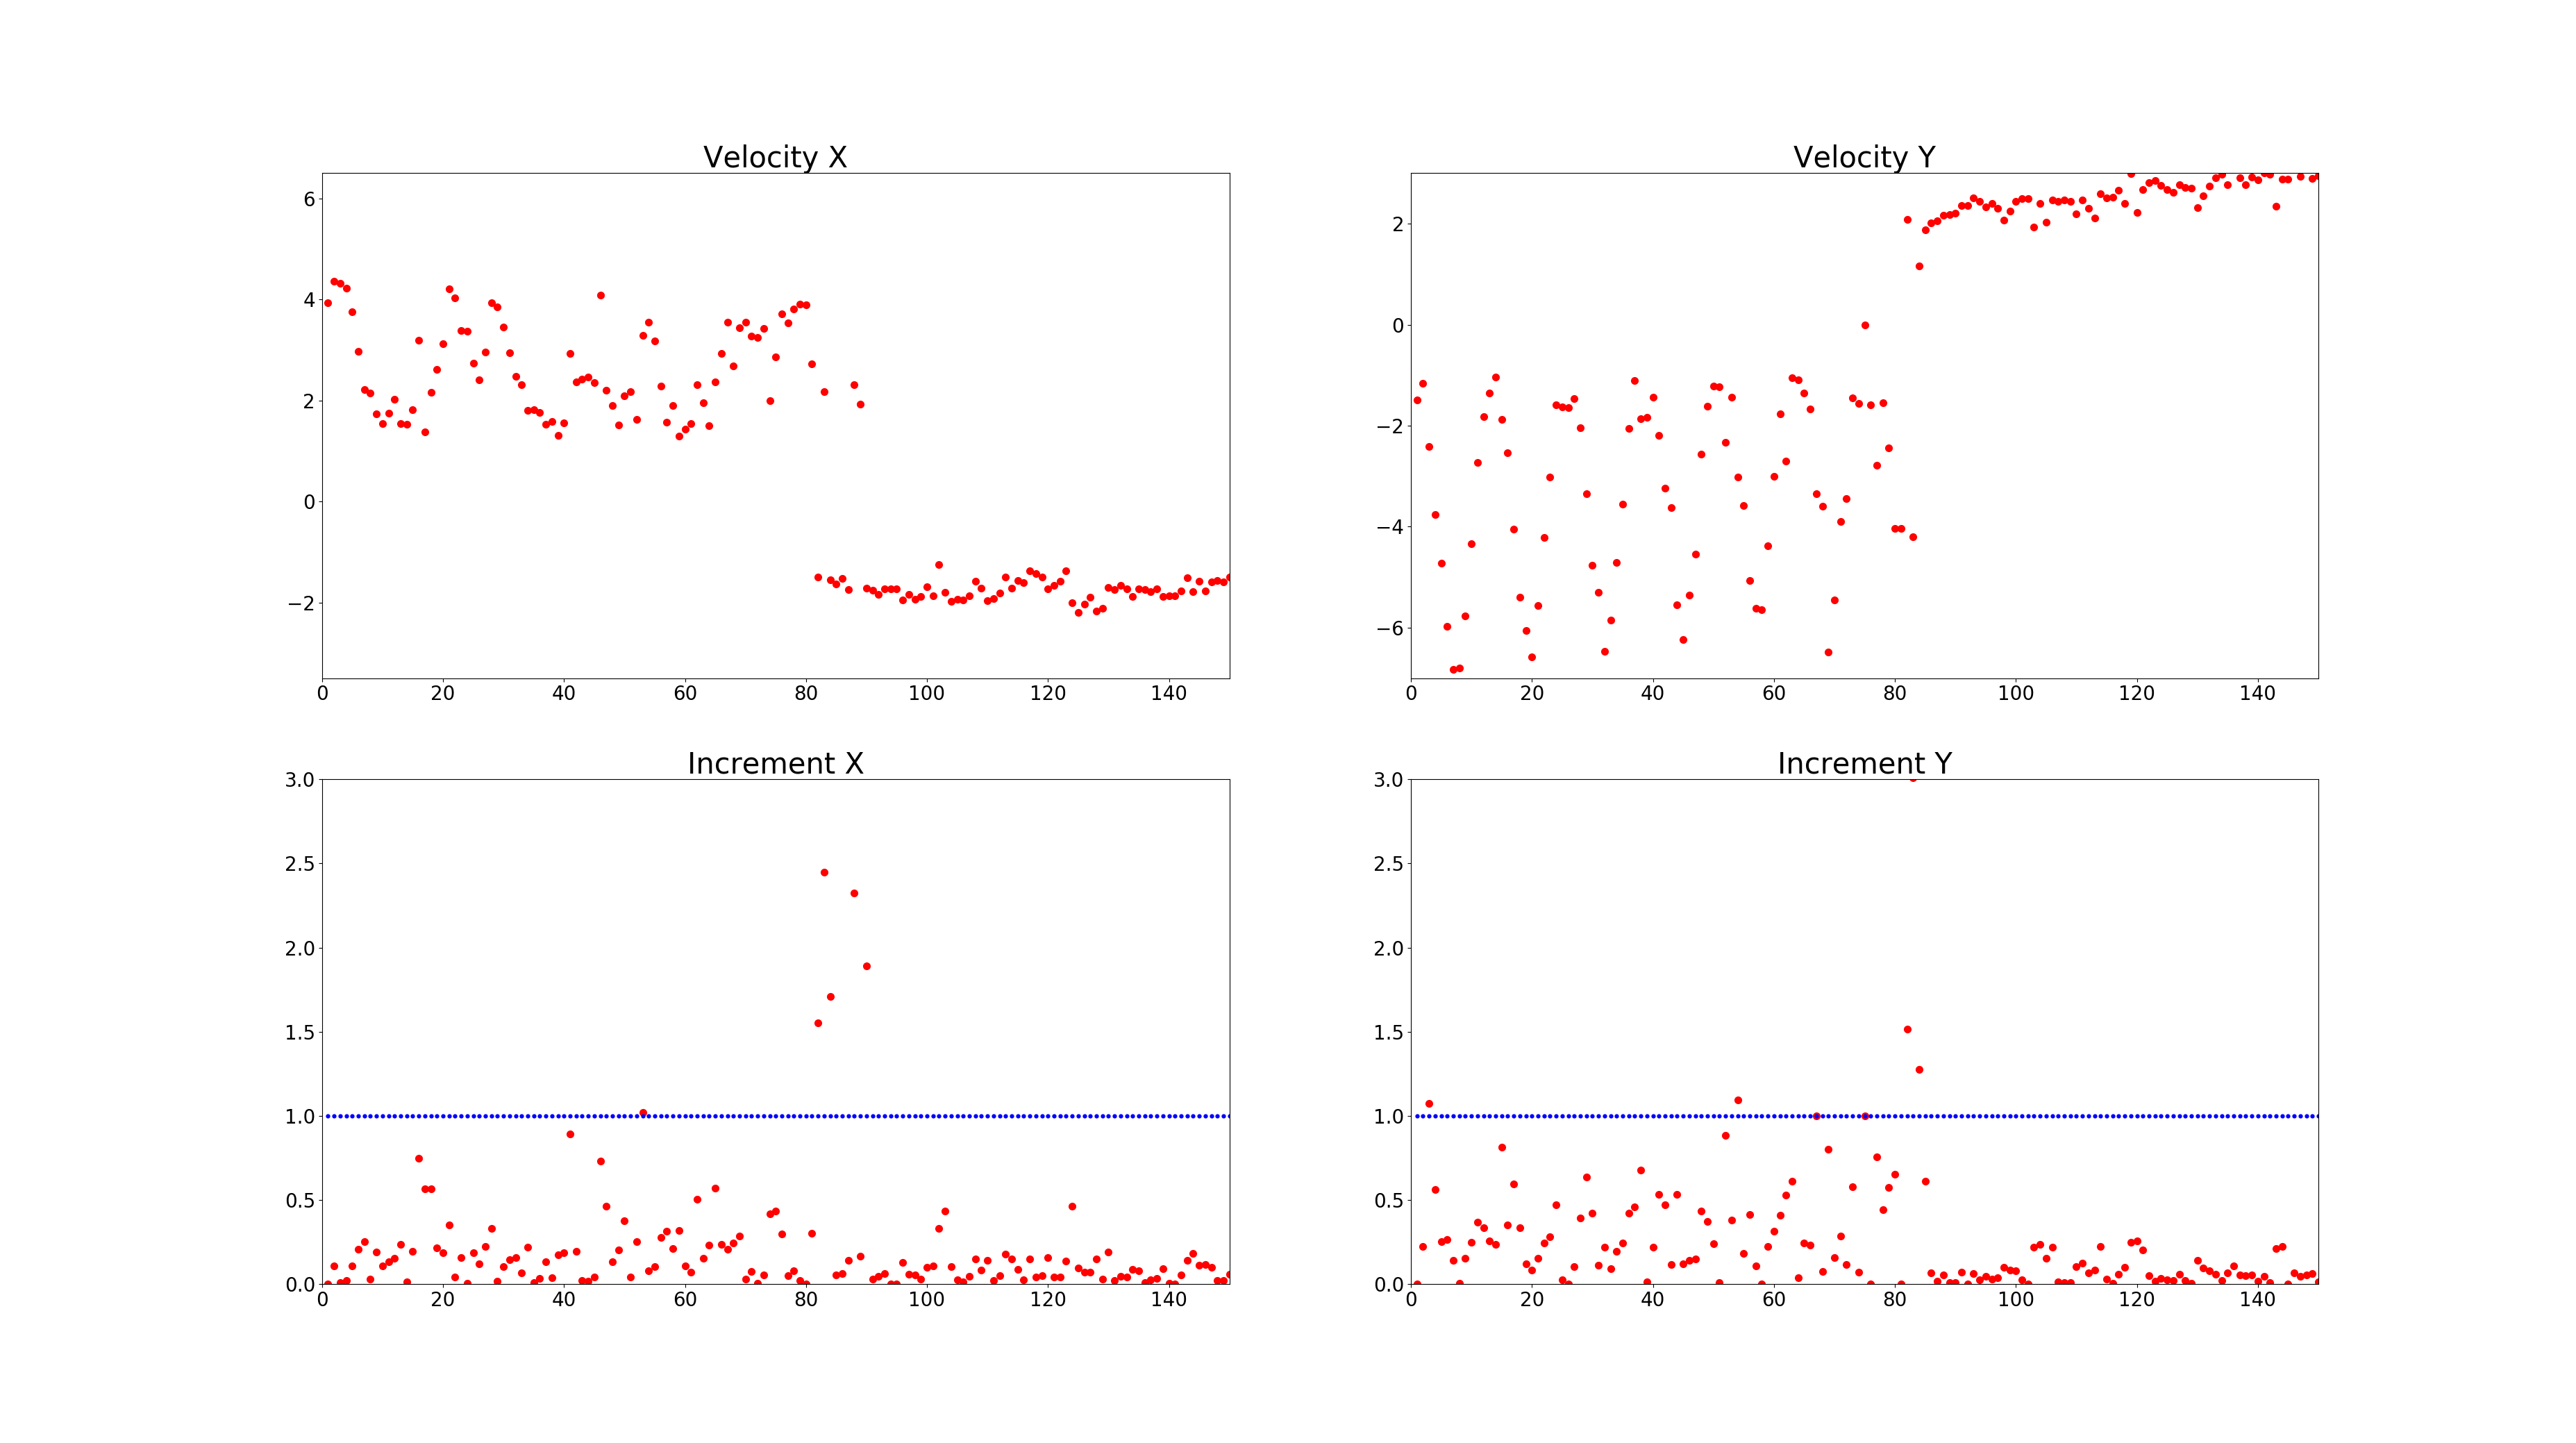
\includegraphics[width=80mm]{velocidadas/bad_threshold.png}}\\

\end{tabular}
\caption{Imatges MRI amb tumor.} \label{pseudo}
\end{figure}





\end{frame}


%\begin{frame}{Tracking success}
%
%
%
%
%
%\begin{figure}[htbp]
%\centering
%\begin{tabular}{ccc}
%\subfloat[Trajectory]{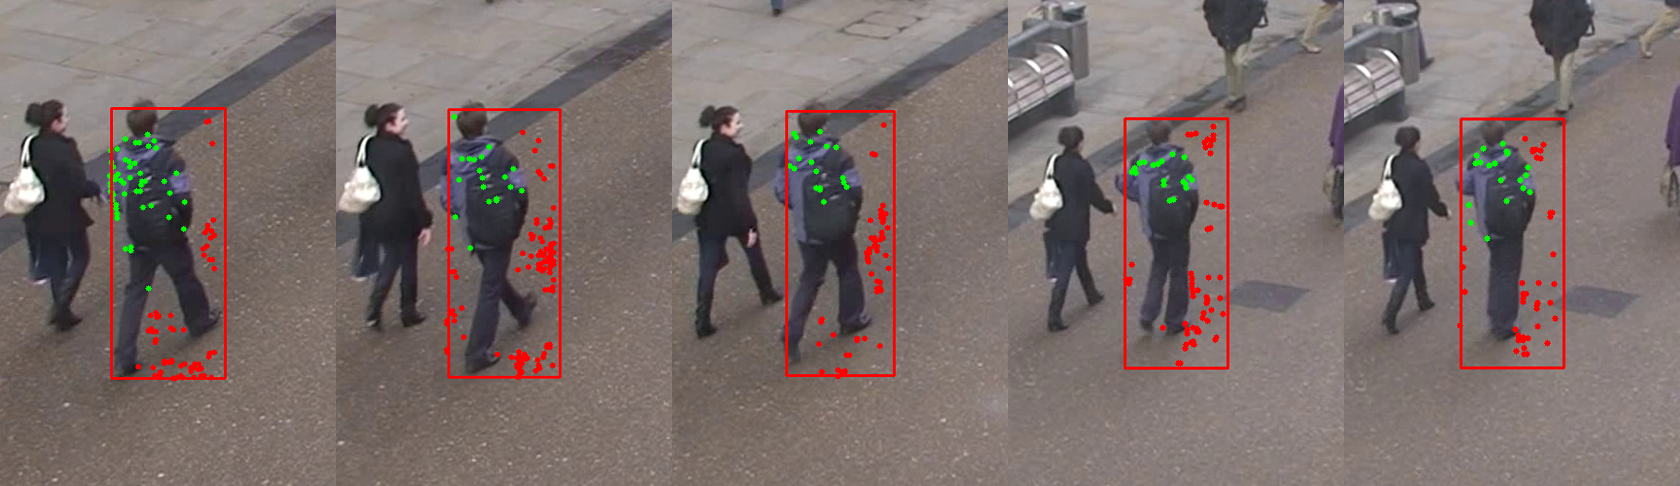
\includegraphics[width=80mm]{velocidadas/tomeuPont.png}}\\
%\subfloat[Plots]{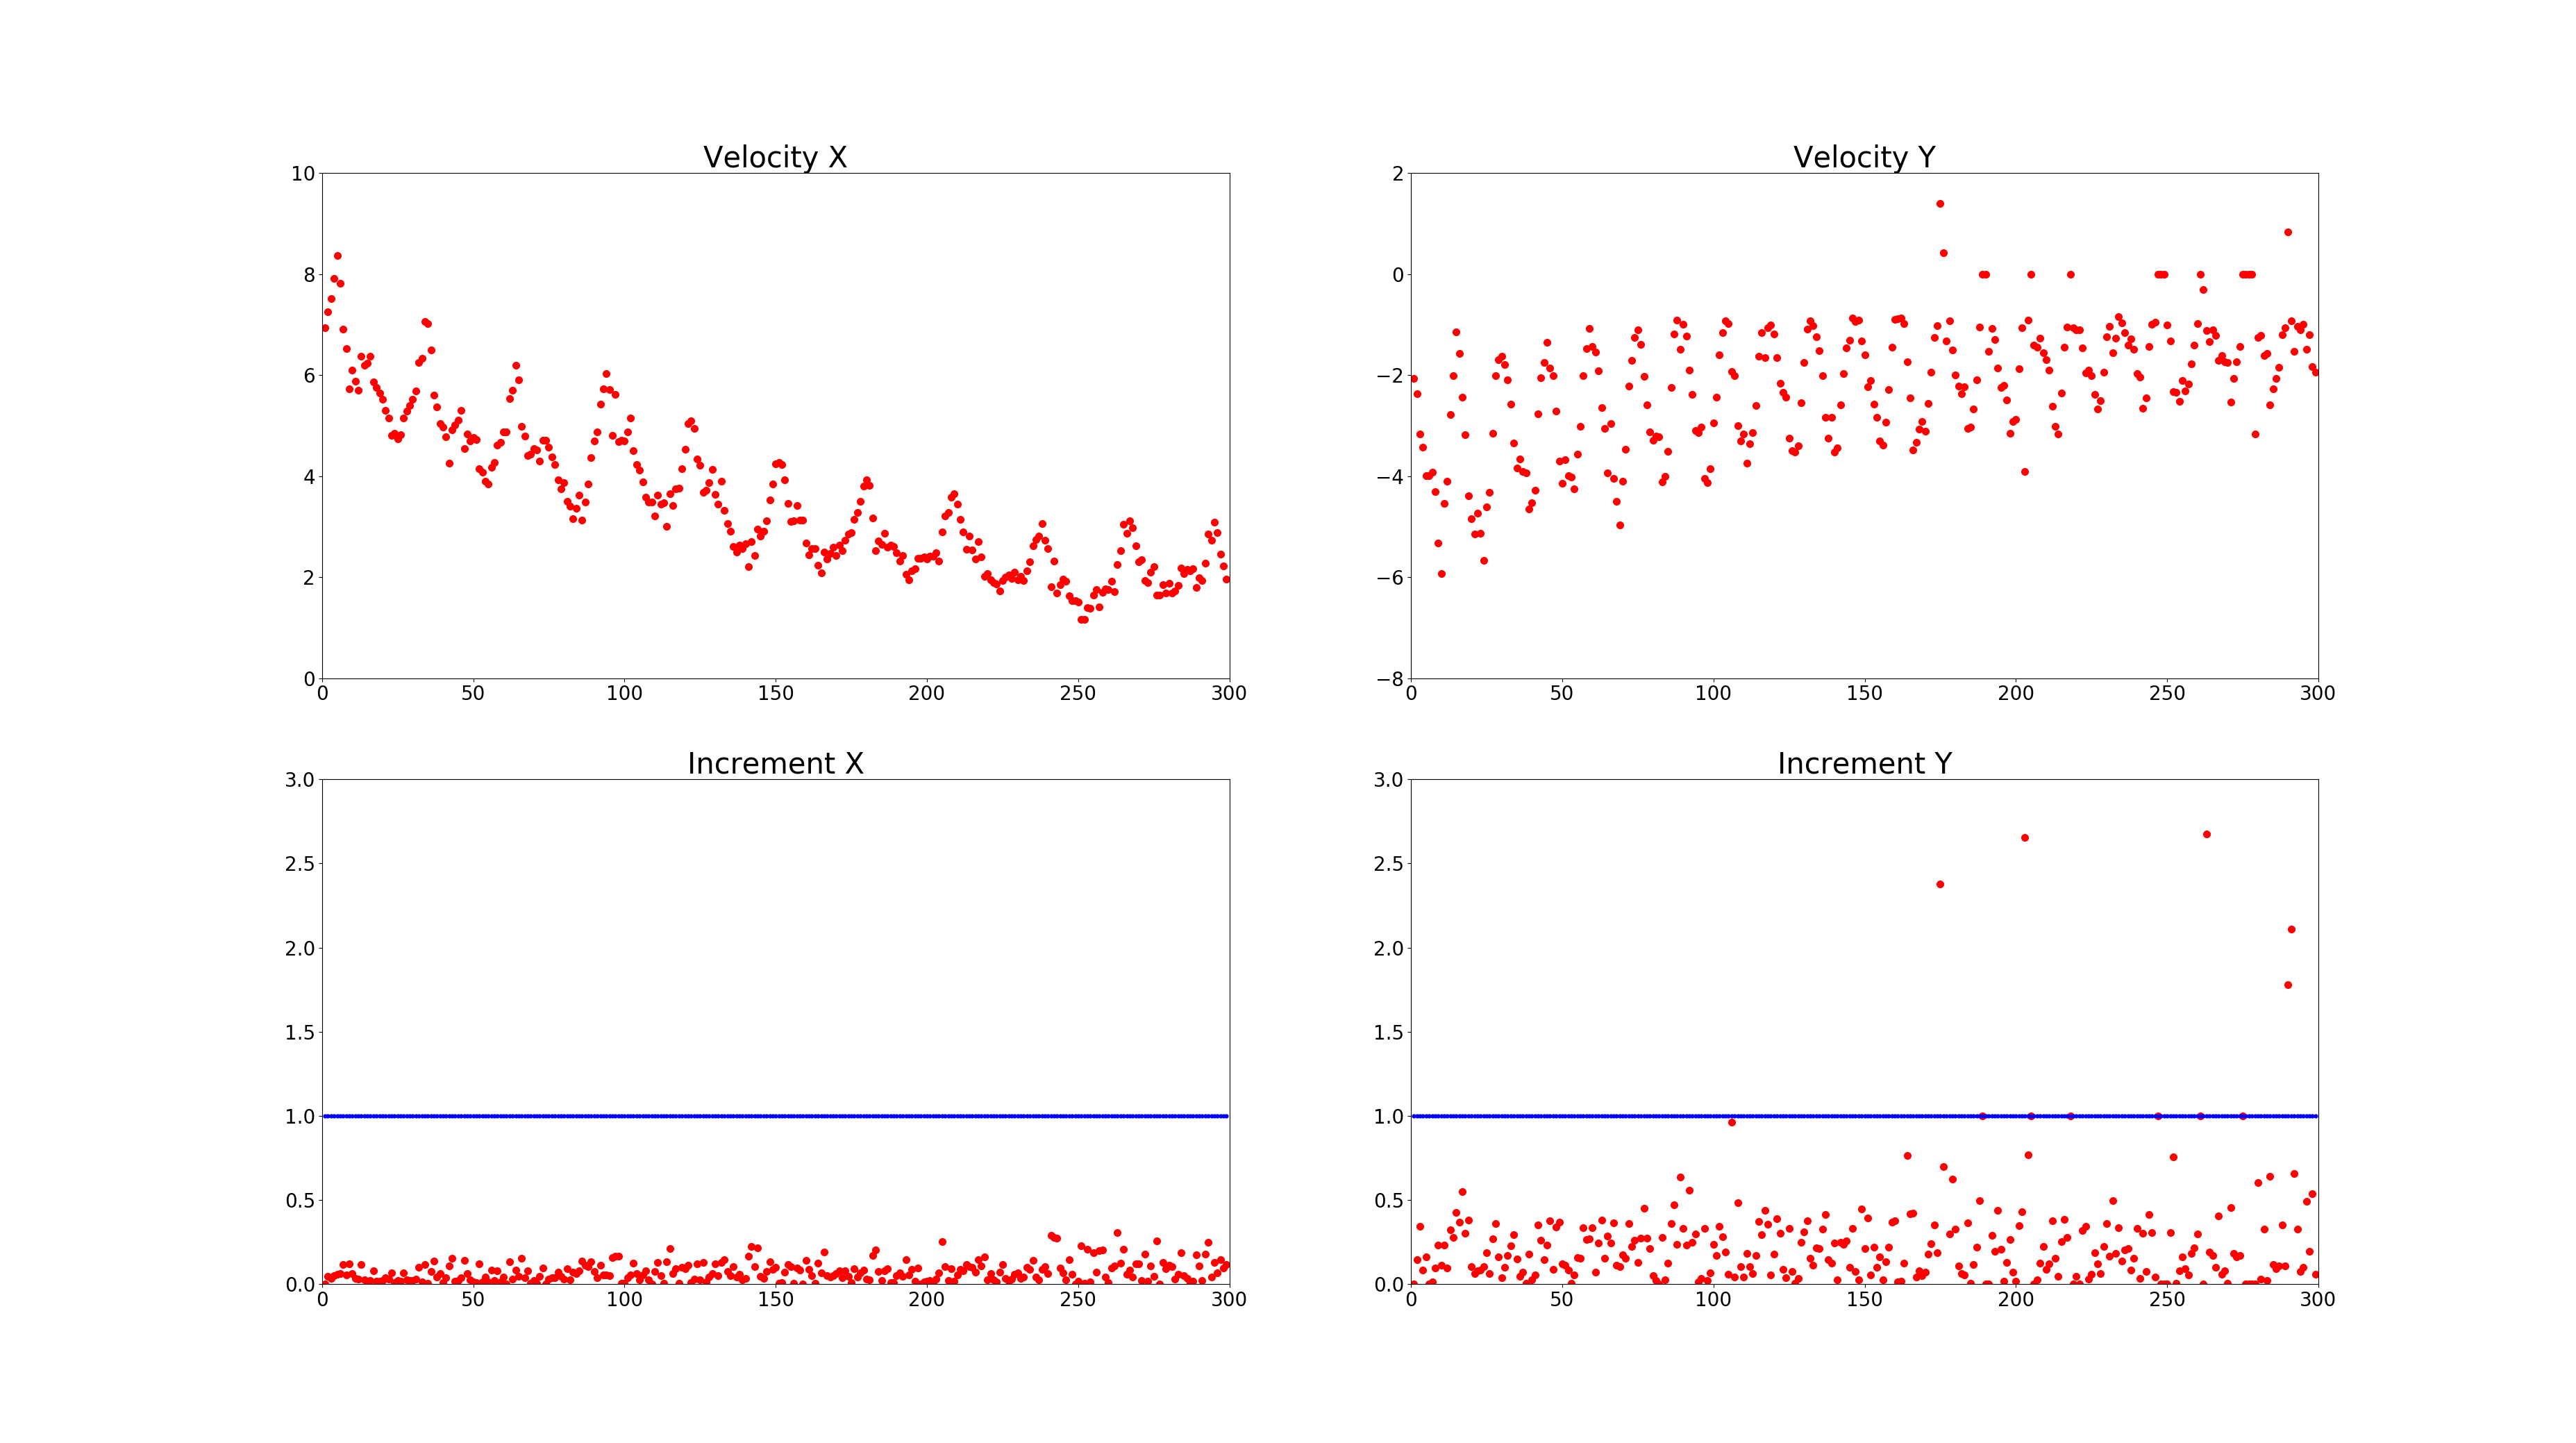
\includegraphics[width=80mm]{velocidadas/good_treshold.png}}\\
%
%\end{tabular}
%\caption{Imatges MRI amb tumor.} \label{pseudo}
%\end{figure}
%
%
%
%
%
%\end{frame}

\subsection{Data Association}

\begin{frame}{Data Association I}

\begin{itemize}



\item \textbf{Situation 1}, blob with nearby detection, replaced by blob detection.

\hspace{2cm}

\item \textbf{Situation 2}, blob without nearby detection, blob continues.


\hspace{2cm}

\item \textbf{Situation 3}, blob detection, new or past ?
\end{itemize}


\end{frame}

\begin{frame}{Data Association II}



\begin{figure}[htbp]
\centering
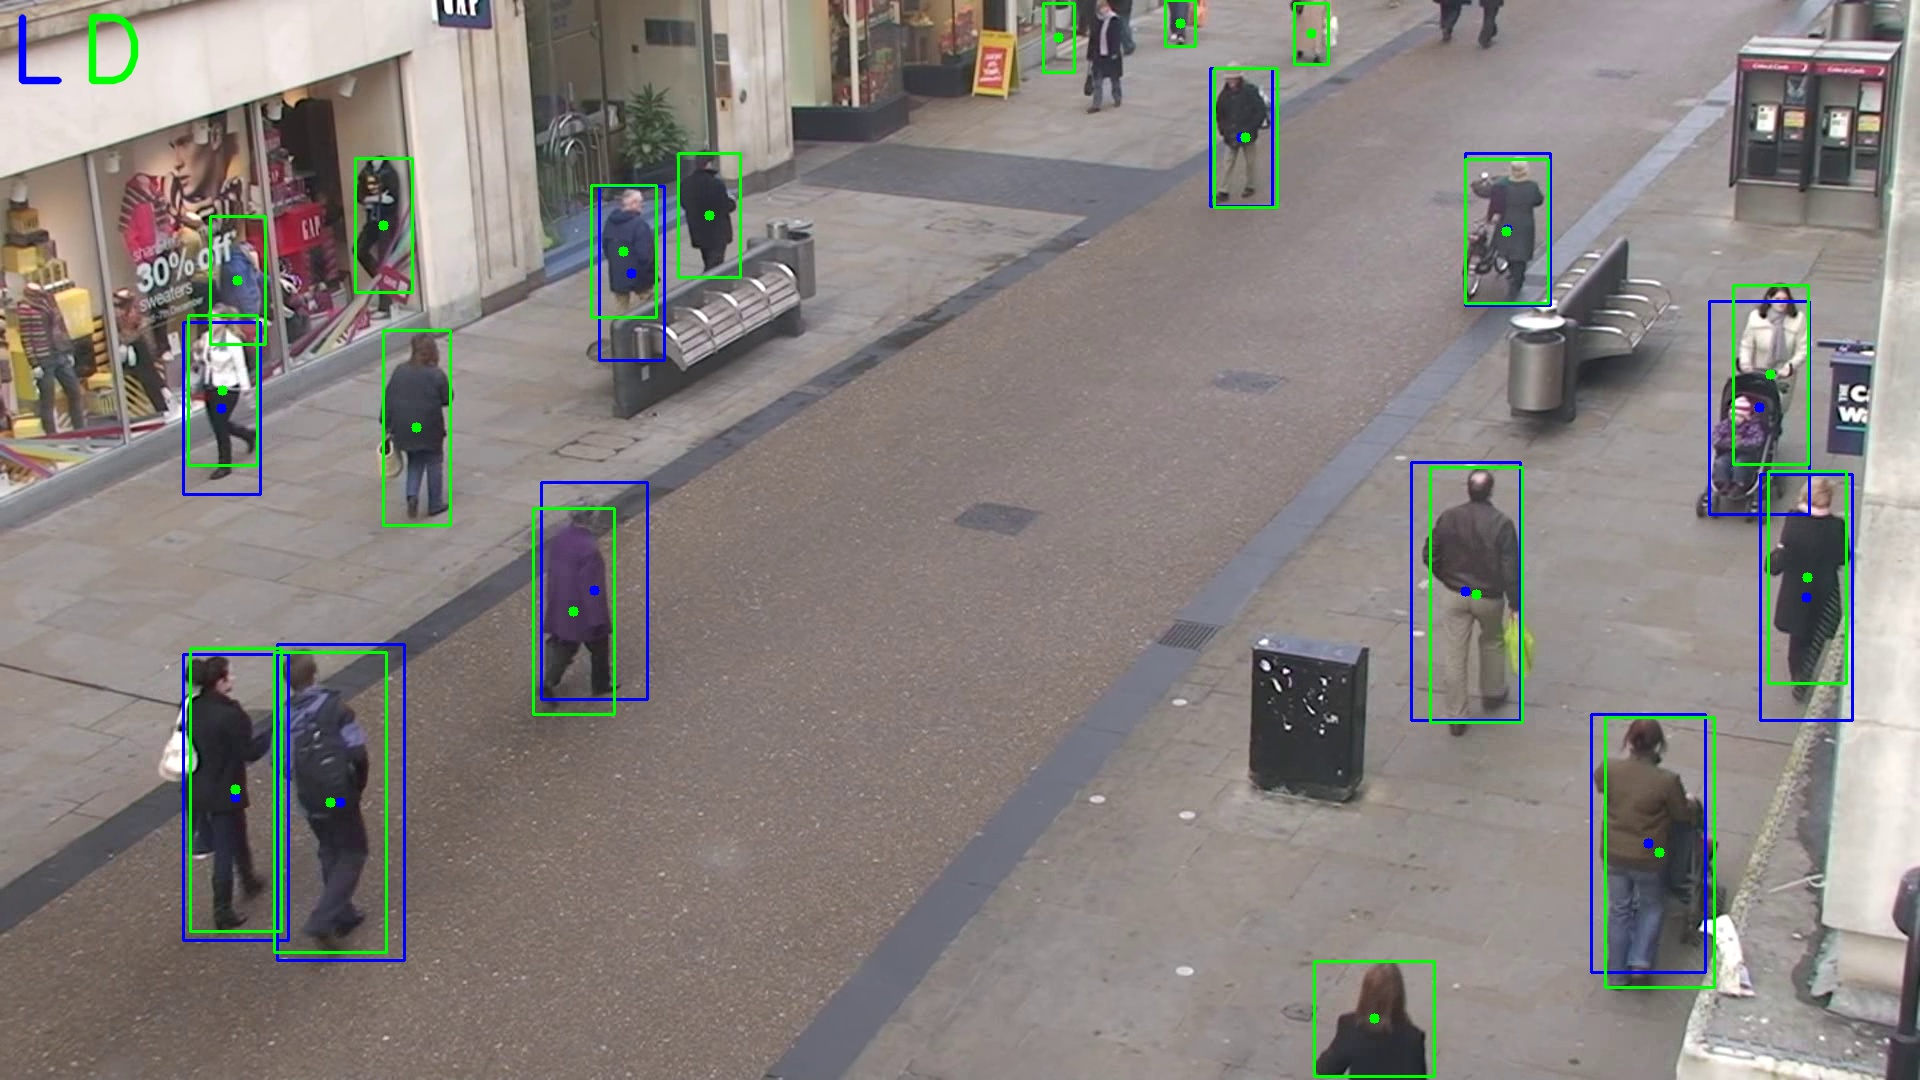
\includegraphics[width=120mm]{./tracker/dataAssociation.jpg}

\end{figure}


\end{frame}

\begin{frame}{Data Association: Siamese architecture}



\begin{figure}[htbp]
\centering
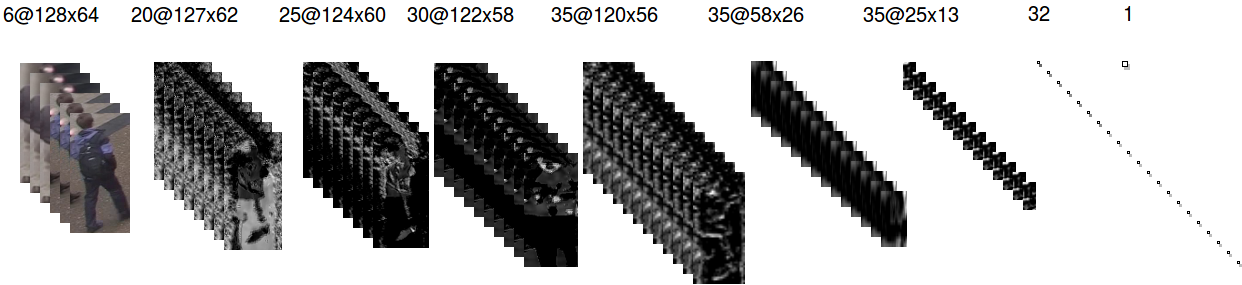
\includegraphics[width=120mm]{./tracker/network6conv.png}

\end{figure}


\end{frame}




\section{Experiments}
%
%\begin{frame}{Object detectors with deep learning}
%
%
%
%\begin{figure}[htbp]
%\centering
%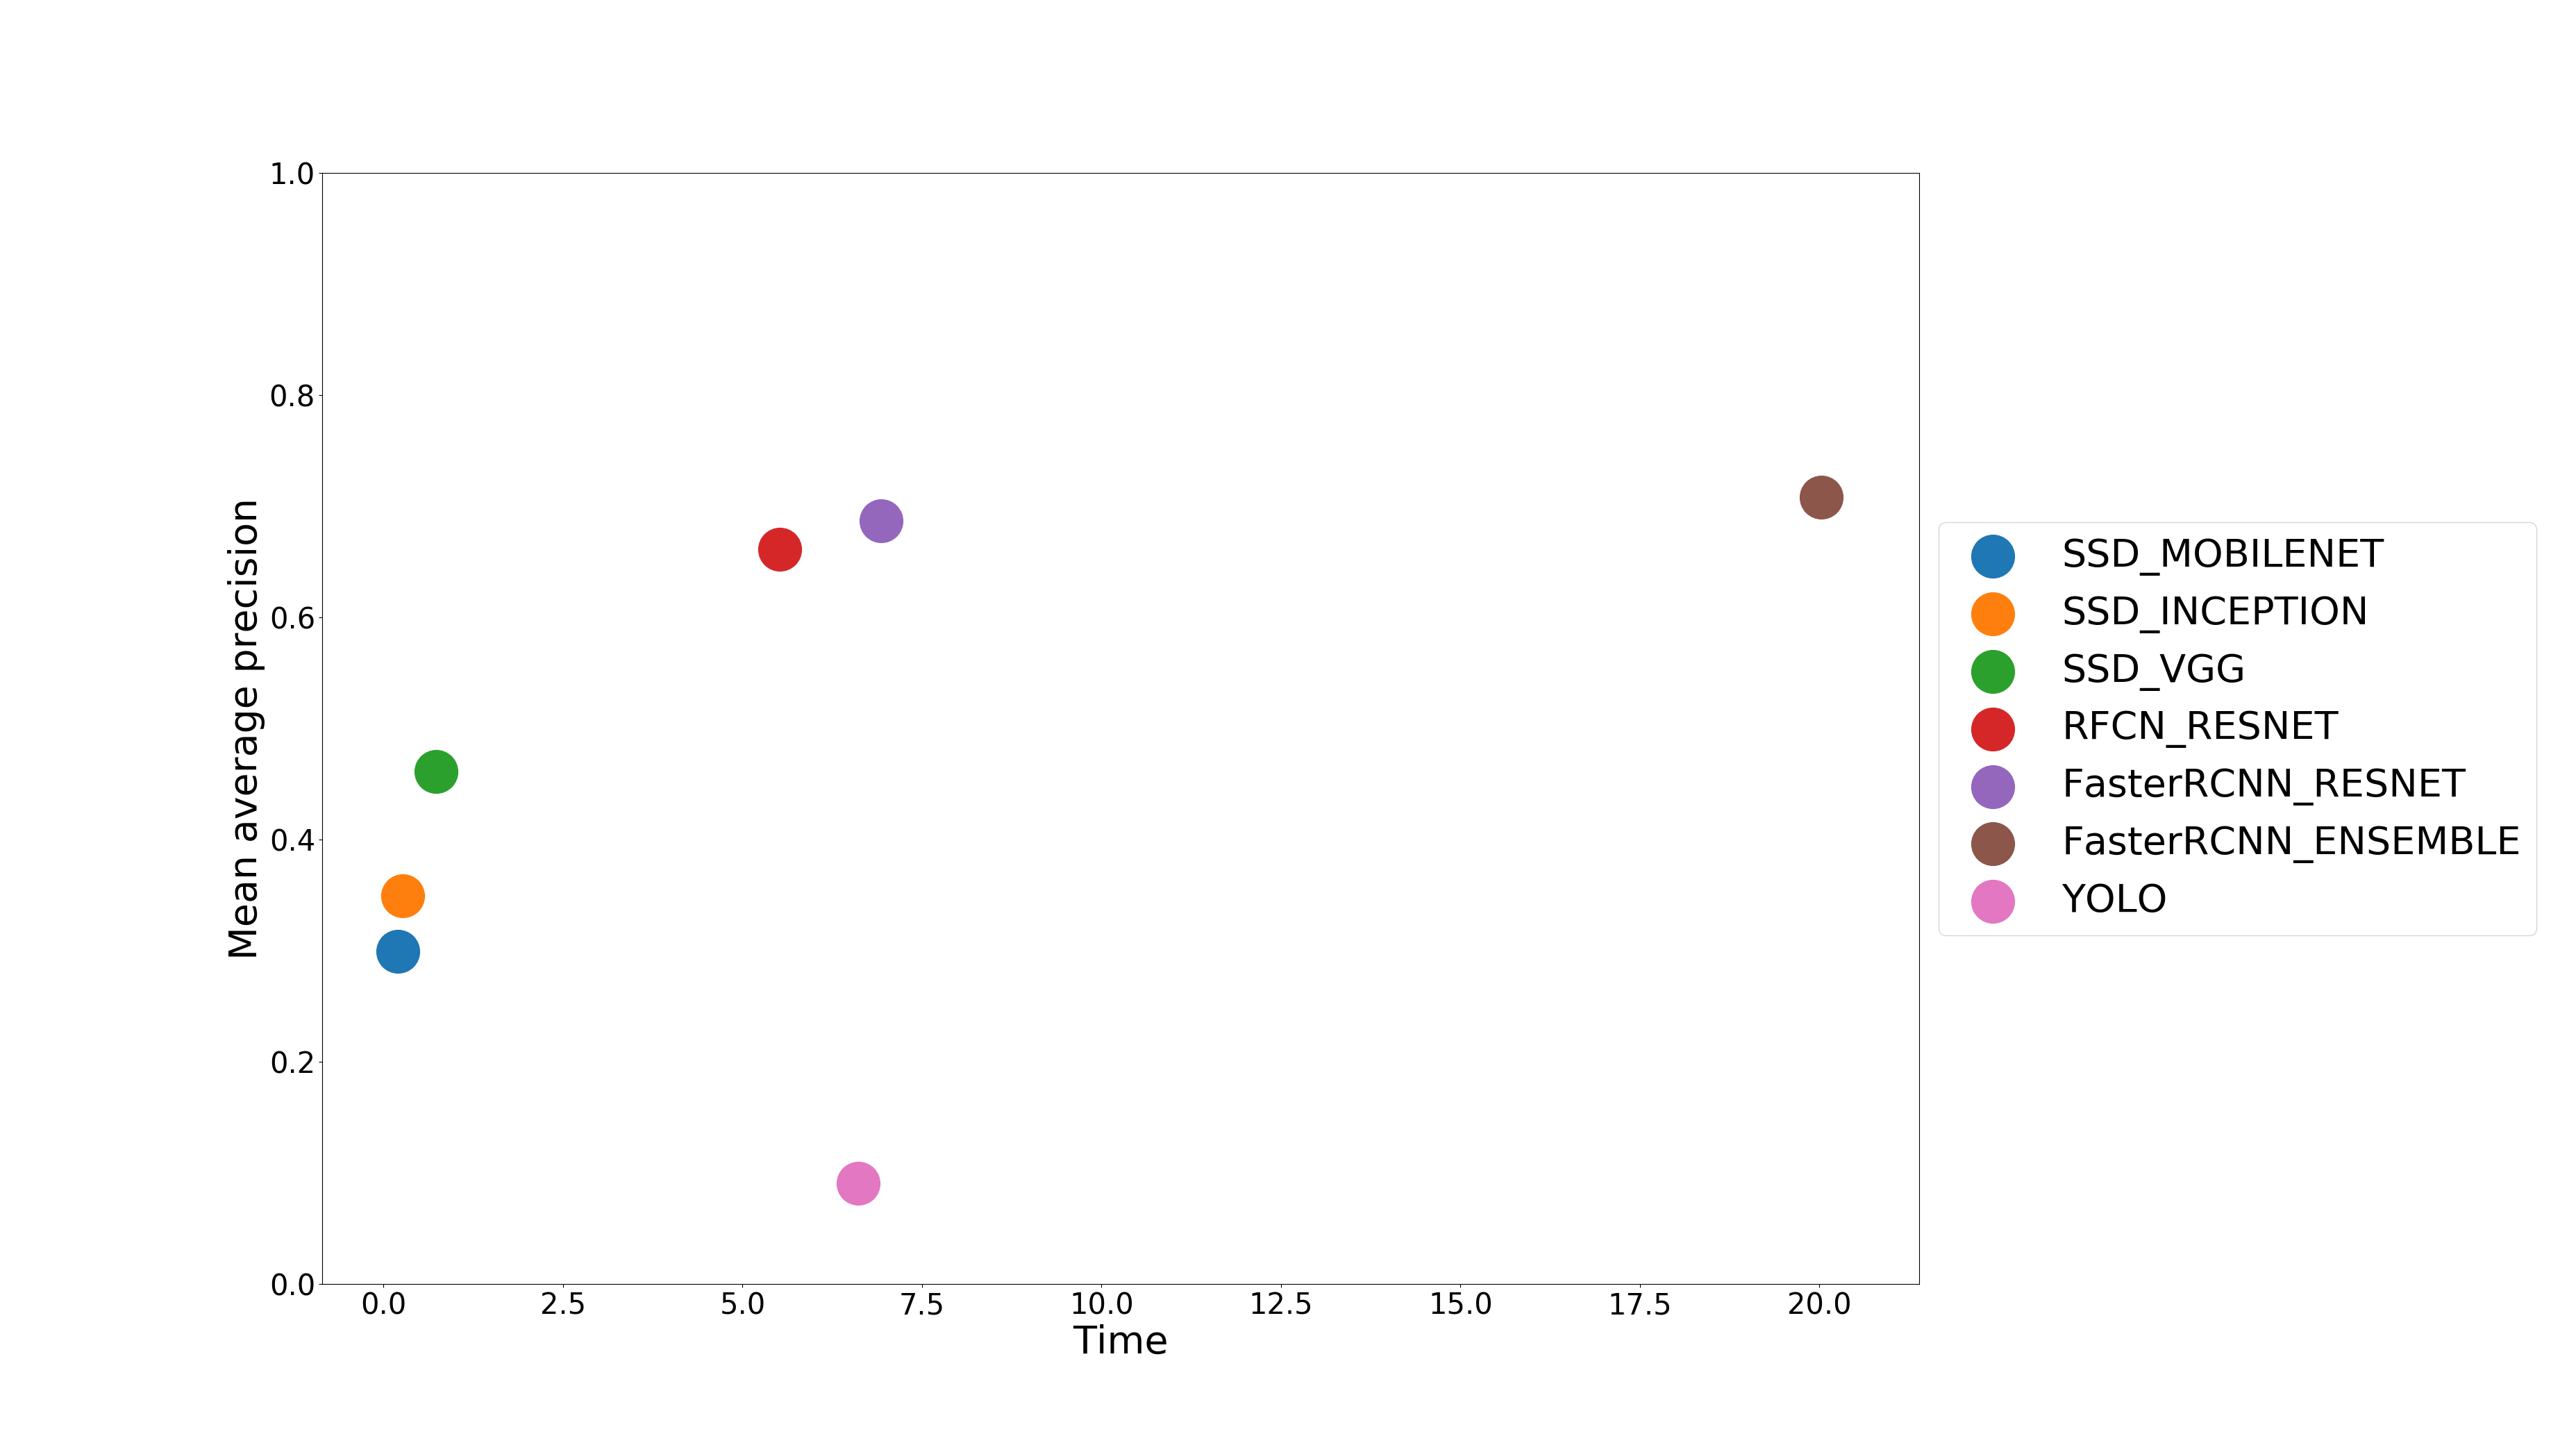
\includegraphics[width=120mm]{./objectdetector/meanAverage2.png}
%
%\end{figure}
%
%
%\end{frame}




\begin{frame}{Reidentification architectures}



\begin{figure}[htbp]
\centering
\begin{tabular}{ccccc}
\subfloat[Cost Function]{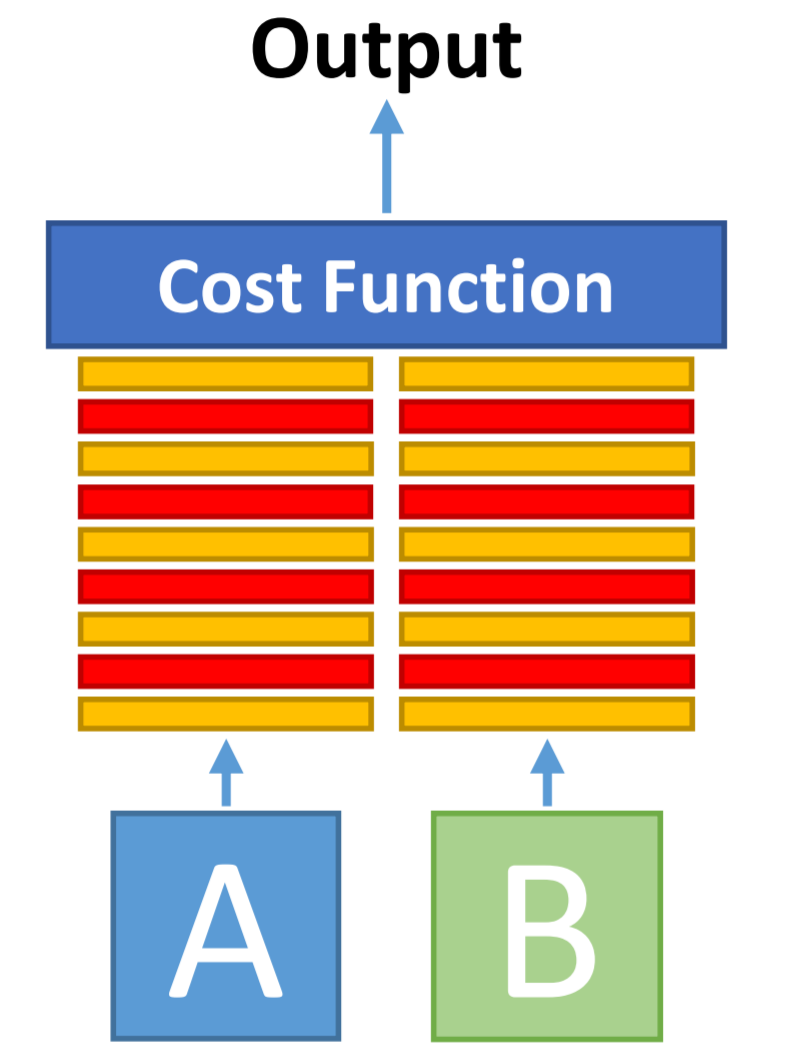
\includegraphics[width=18mm]{siamese/retall1.png}}&
\subfloat[In-Network]{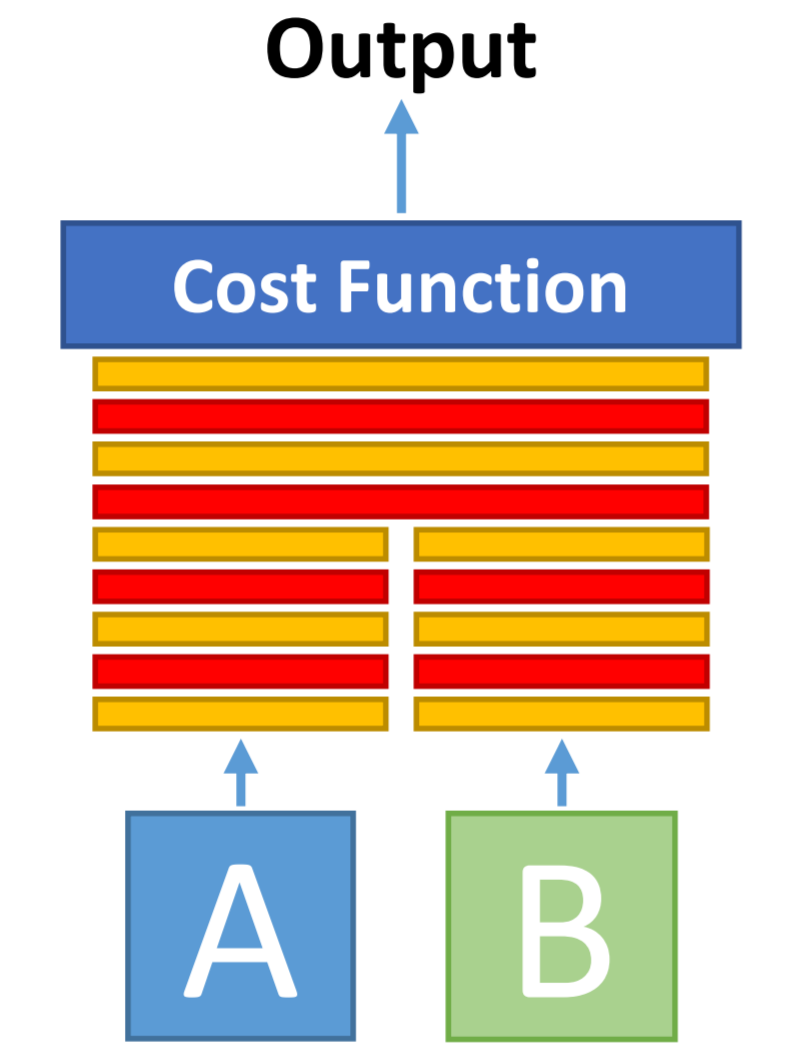
\includegraphics[width=18mm]{siamese/retall2.png}}&
\subfloat[Joint data input]{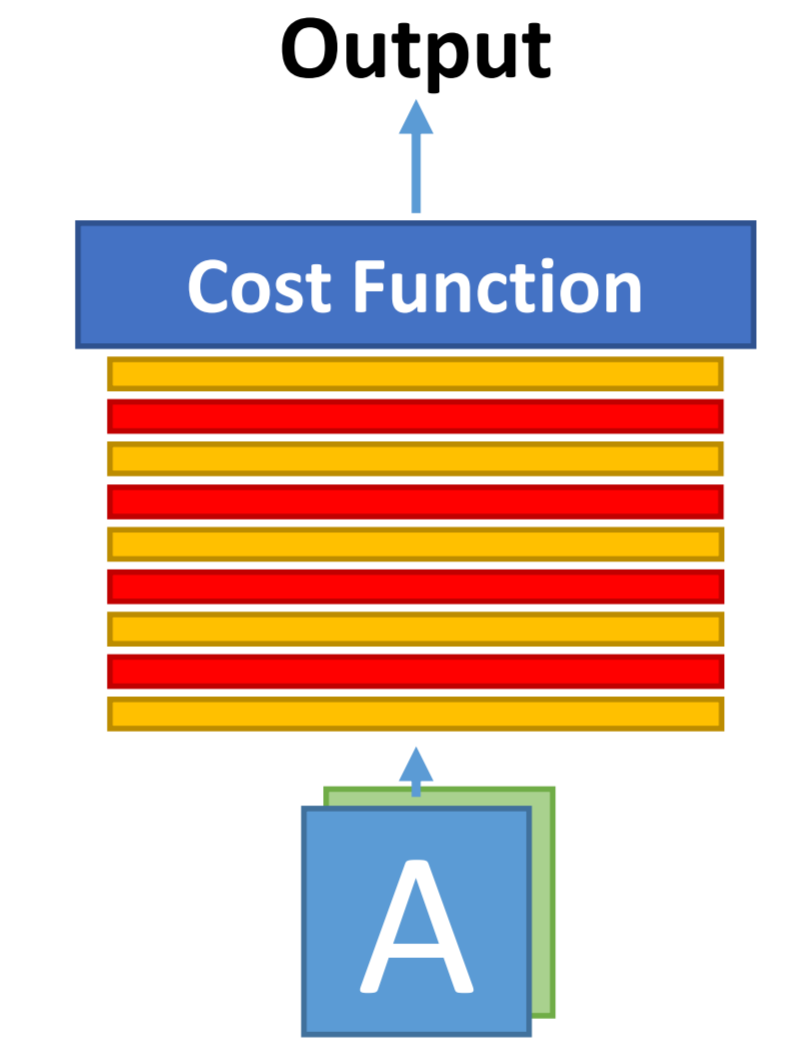
\includegraphics[width=18mm]{siamese/retall3.png}}&
\subfloat[Feature extractor with cosine distance]{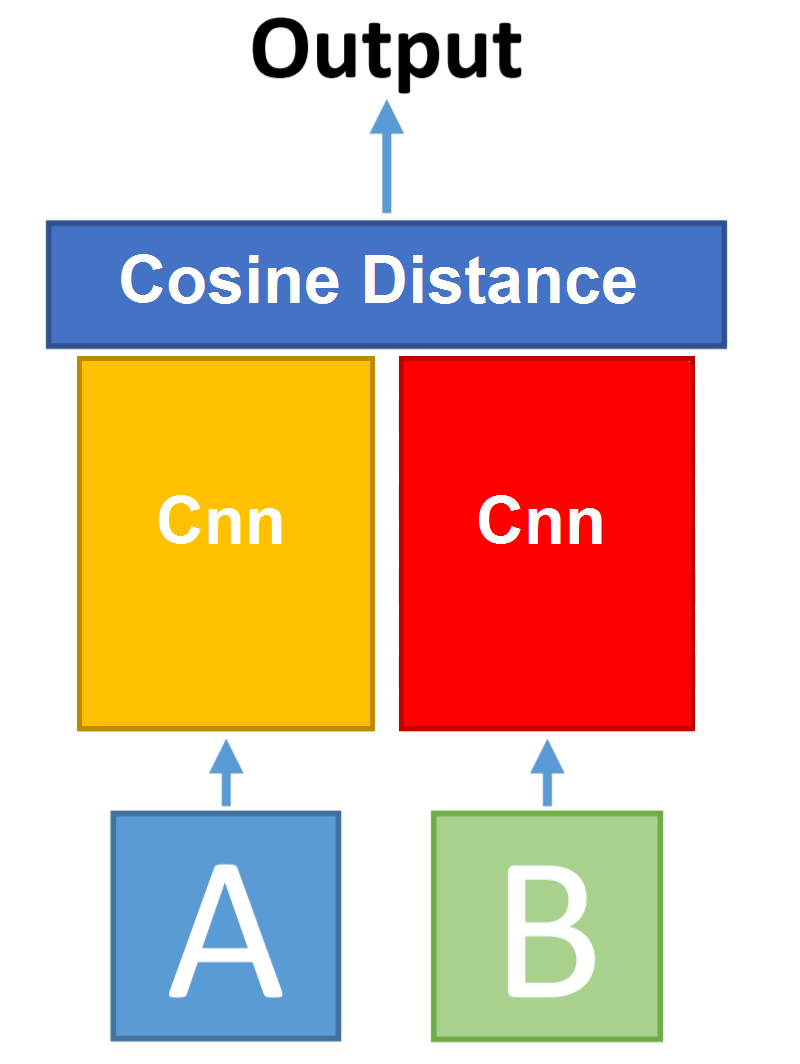
\includegraphics[width=18mm]{siamese/cosineDistance.png}}&
\subfloat[Feature network fine-tuned]{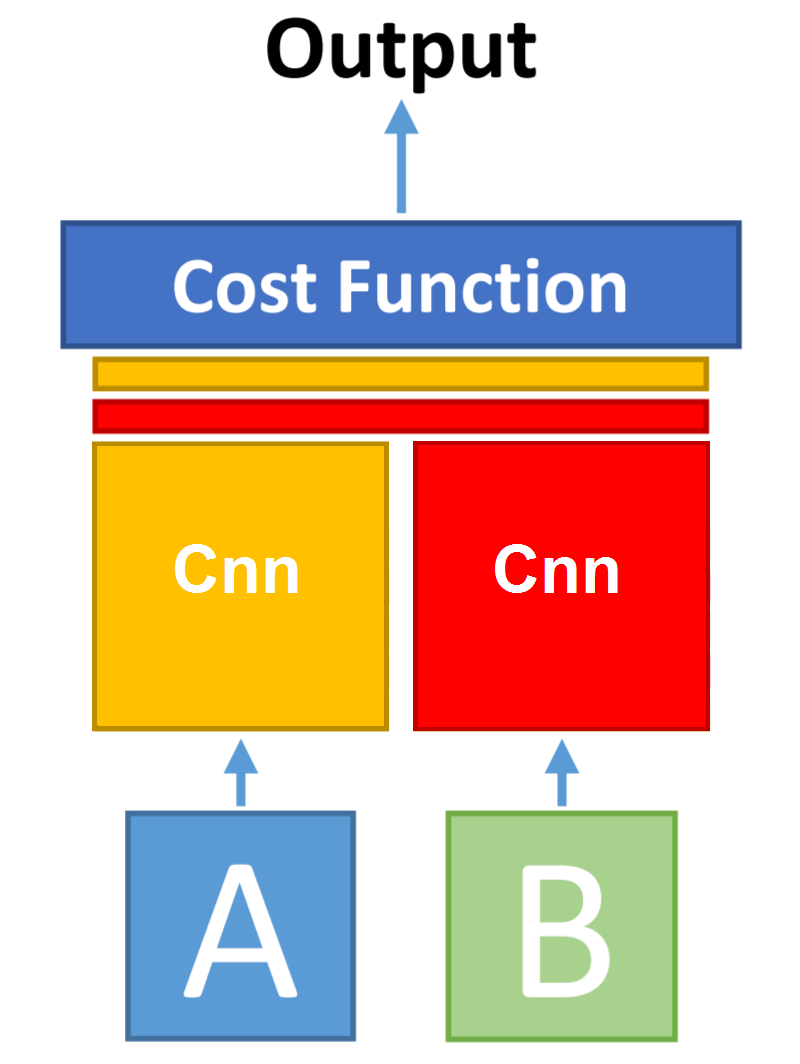
\includegraphics[width=18mm]{siamese/retall2cnnMAss.png}}\\


\end{tabular}
%\caption{Imatges MRI amb tumor.} \label{pseudo}
\end{figure}


\end{frame}

\begin{frame}{Data augmentation}



\begin{figure}[htbp]
\centering
\begin{tabular}{ccccc}
\subfloat[Original]{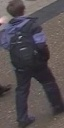
\includegraphics[width=12mm]{augmentation/resizedImage.jpg}}
\subfloat[Random brightness]{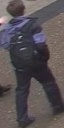
\includegraphics[width=12mm]{augmentation/imageBrightnes.jpg}}
\subfloat[Random crop]{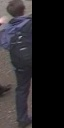
\includegraphics[width=12mm]{augmentation/imageRandomCrop.jpg}}
\subfloat[Vertical flip]{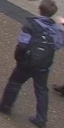
\includegraphics[width=12mm]{augmentation/imageVerticalFlip.jpg}}
\subfloat[Gaussian blur]{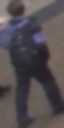
\includegraphics[width=12mm]{augmentation/imageGaussianBlur.jpg}}
\subfloat[Random shadow]{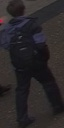
\includegraphics[width=12mm]{augmentation/imageRandomShadow.jpg}}\\

\subfloat[Zoom in]{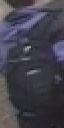
\includegraphics[width=12mm]{augmentation/imageZoomIn.jpg}}
\subfloat[Translation and rotation]{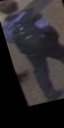
\includegraphics[width=12mm]{augmentation/imageTransormed.jpg}}
\subfloat[Zoom out]{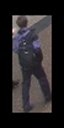
\includegraphics[width=12mm]{augmentation/imageZoomOut.jpg}}
\subfloat[Gaussian noise]{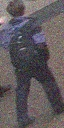
\includegraphics[width=12mm]{augmentation/imageNoiseGaussian.jpg}}
\subfloat[Opposite Vignetting]{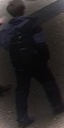
\includegraphics[width=12mm]{augmentation/imageBLURcenter.jpg}}


\end{tabular}
%\caption{Imatges MRI amb tumor.} \label{pseudo}
\end{figure}



\end{frame}

%
\begin{frame}{Parameters training network I}


\begin{itemize}

\item \textbf{Loss}: Binary cross entropy.

\vspace{0.75cm}

\item \textbf{Optimizer}: Adam with exponential decay.

\vspace{0.75cm}

\item \textbf{Activation}: ReLu. 

\vspace{0.75cm}

\item \textbf{Initialization}: He. initialization. Biases with the value of $0.1$.

\vspace{0.75cm}

\item \textbf{Regularization}: Dropout in the fully connected layer.



\end{itemize}


\end{frame}


\begin{frame}{Parameters training network II}

\begin{itemize}


\item \textbf{Preprocessing}: Centre the data and normalized.

\item \textbf{Final layers}: Flatten, Global Average Pooling and Spatial pyramid pooling.


\begin{figure}[htbp]
\centering
\begin{tabular}{ccc}
\subfloat[Flatten]{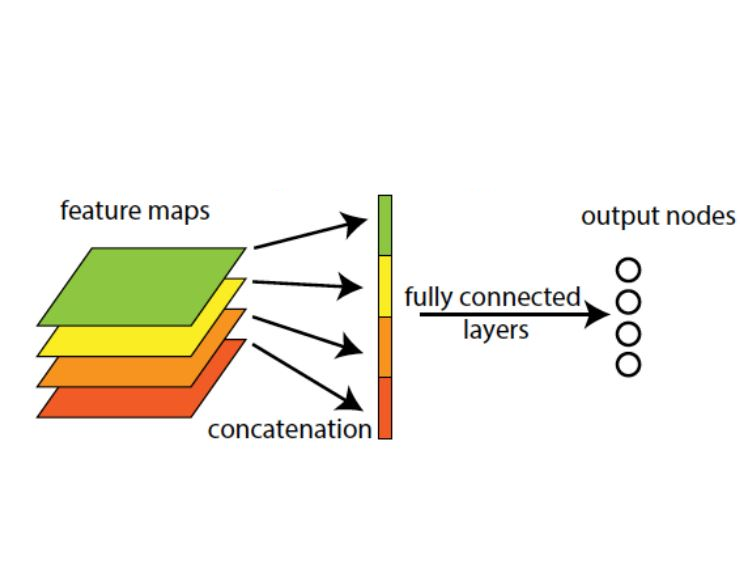
\includegraphics[width=30mm]{siameseLayers/flatten2.png}}
\subfloat[Global Average Pooling]{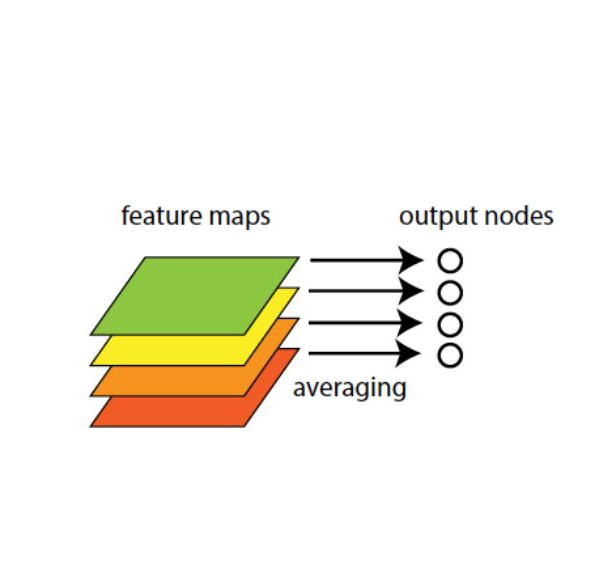
\includegraphics[width=25mm]{siameseLayers/global2.png}}




\end{tabular}
%\caption{Imatges MRI amb tumor.} \label{pseudo}
\end{figure}


\item \textbf{Output}: Sigmoid activation.


\end{itemize}



\end{frame}


%\begin{frame}{Results training}
%
%\begin{figure}[htbp]
%\centering
%\begin{tabular}{cc}
%\subfloat[Loss in training]{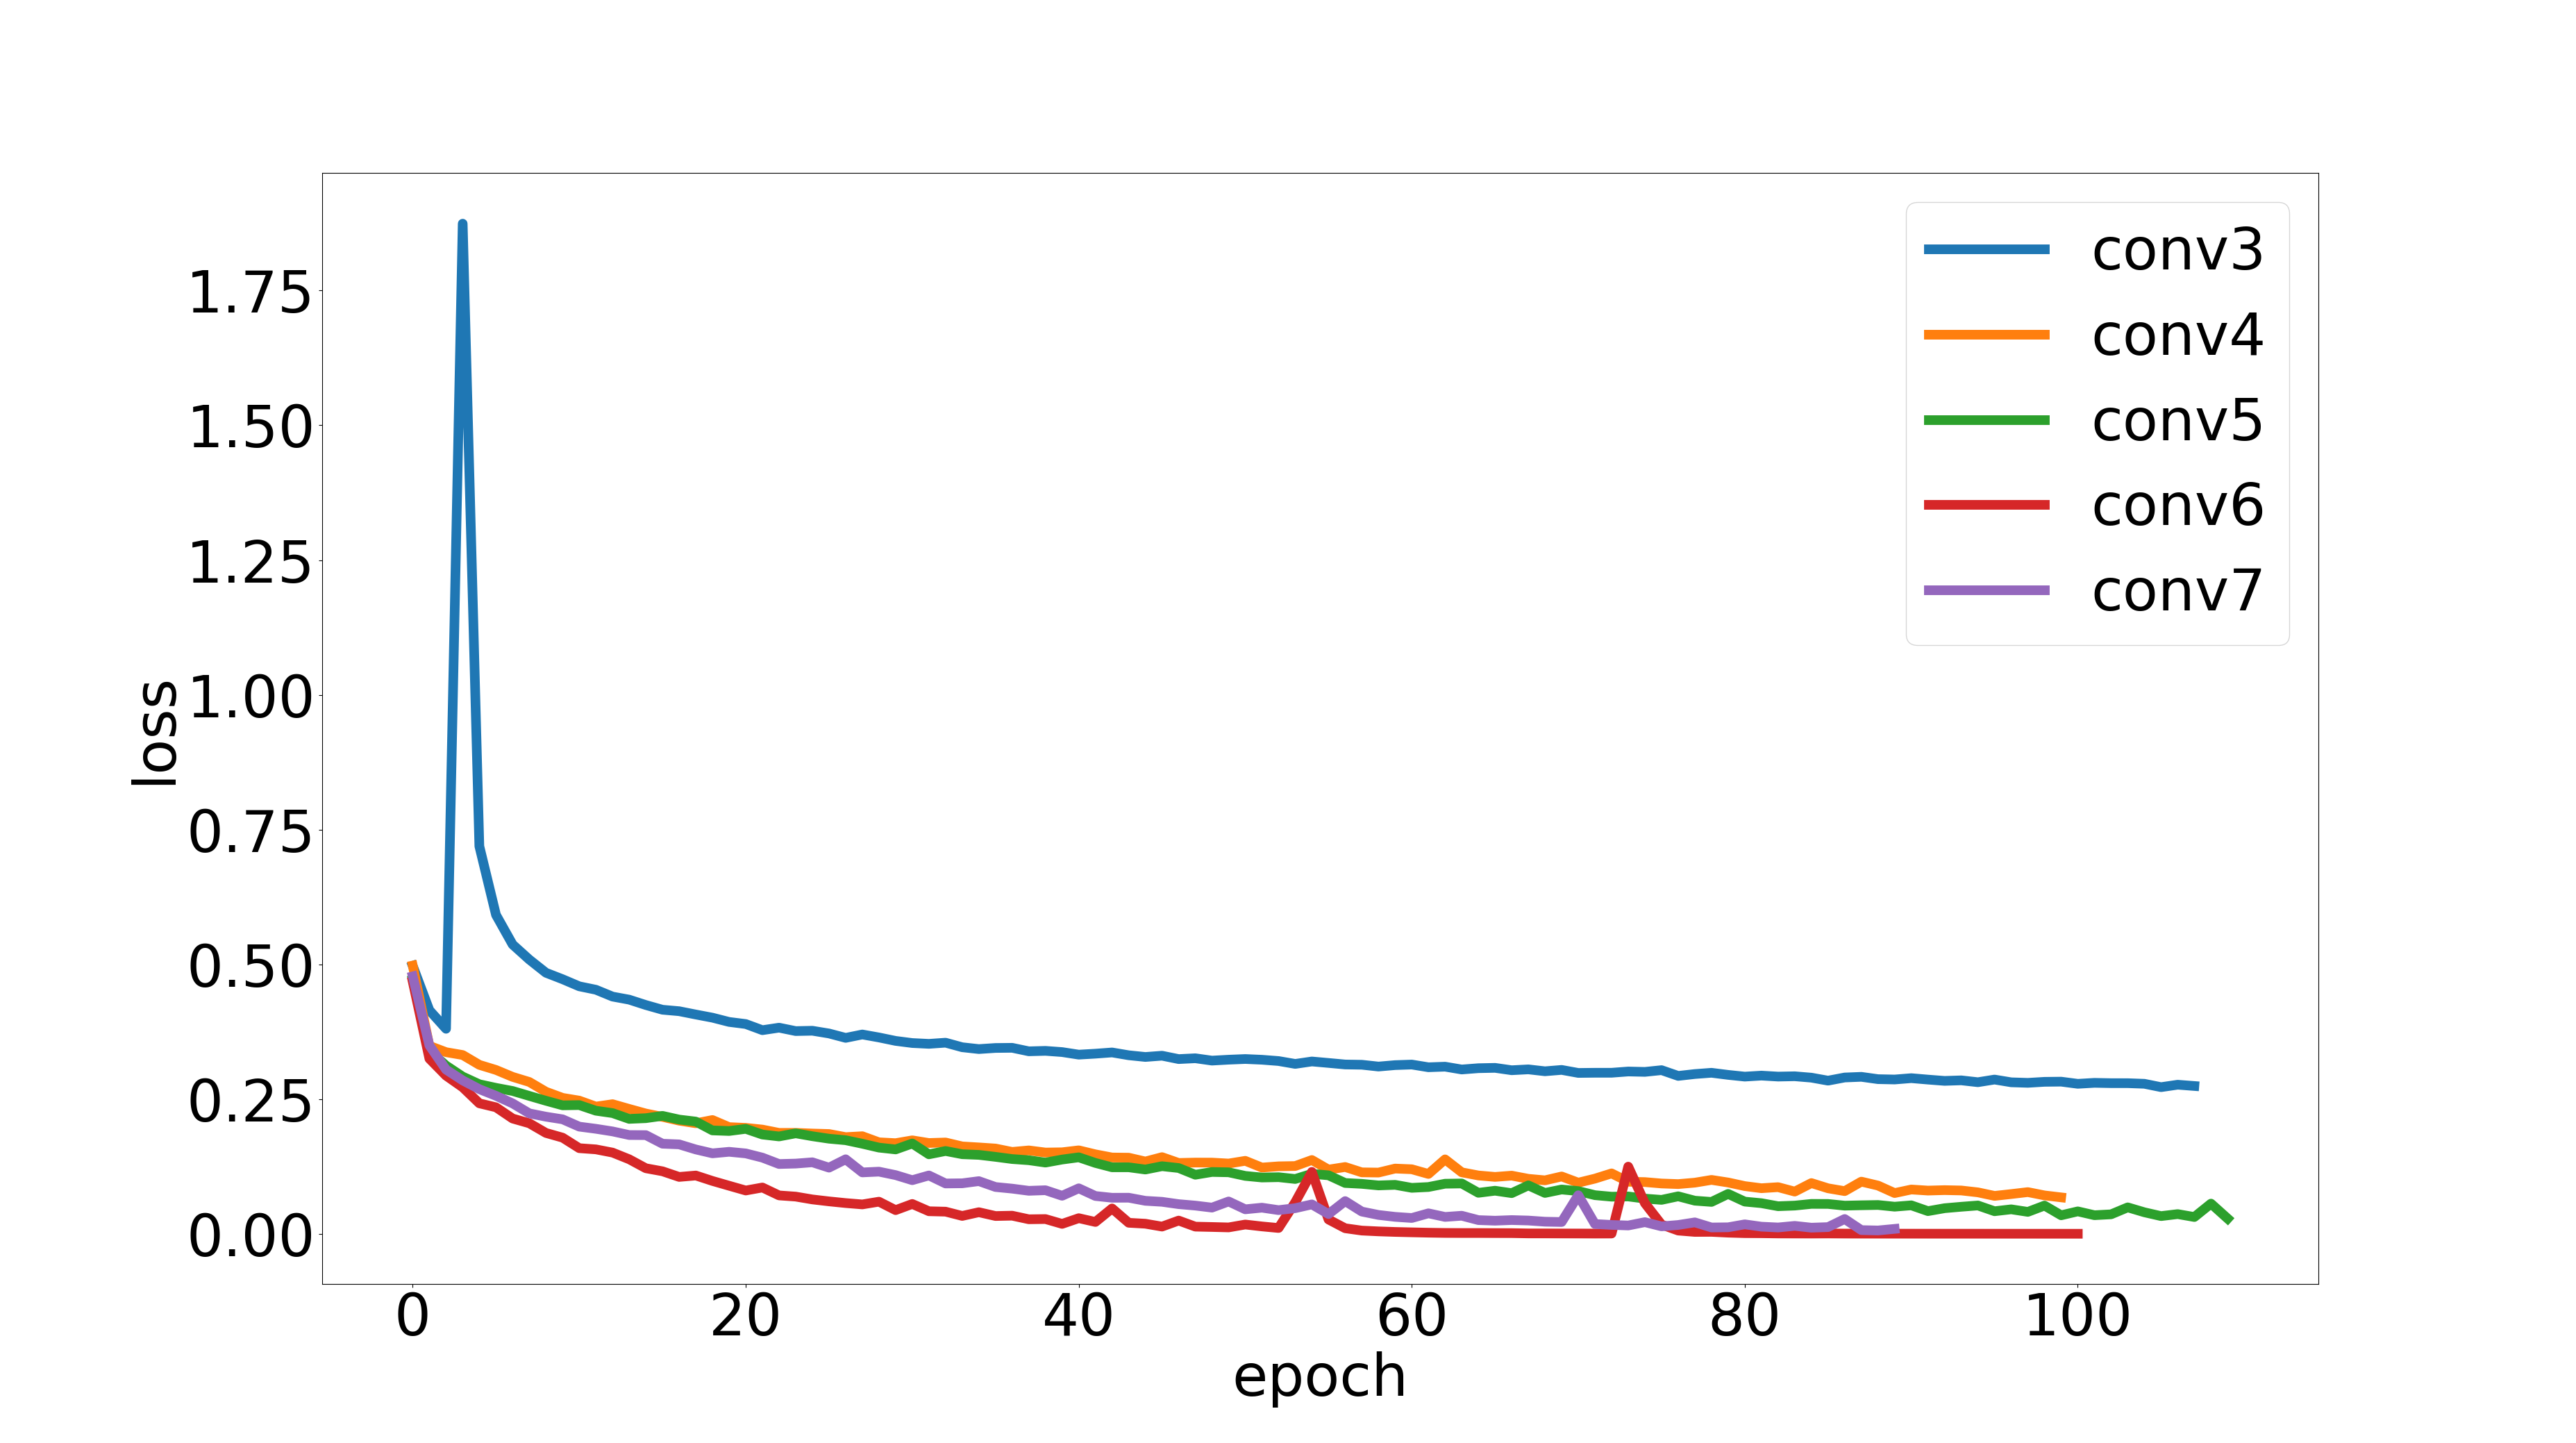
\includegraphics[width=55mm]{siameseLayers/train-loss.png}}
%\subfloat[Accuracy in training]{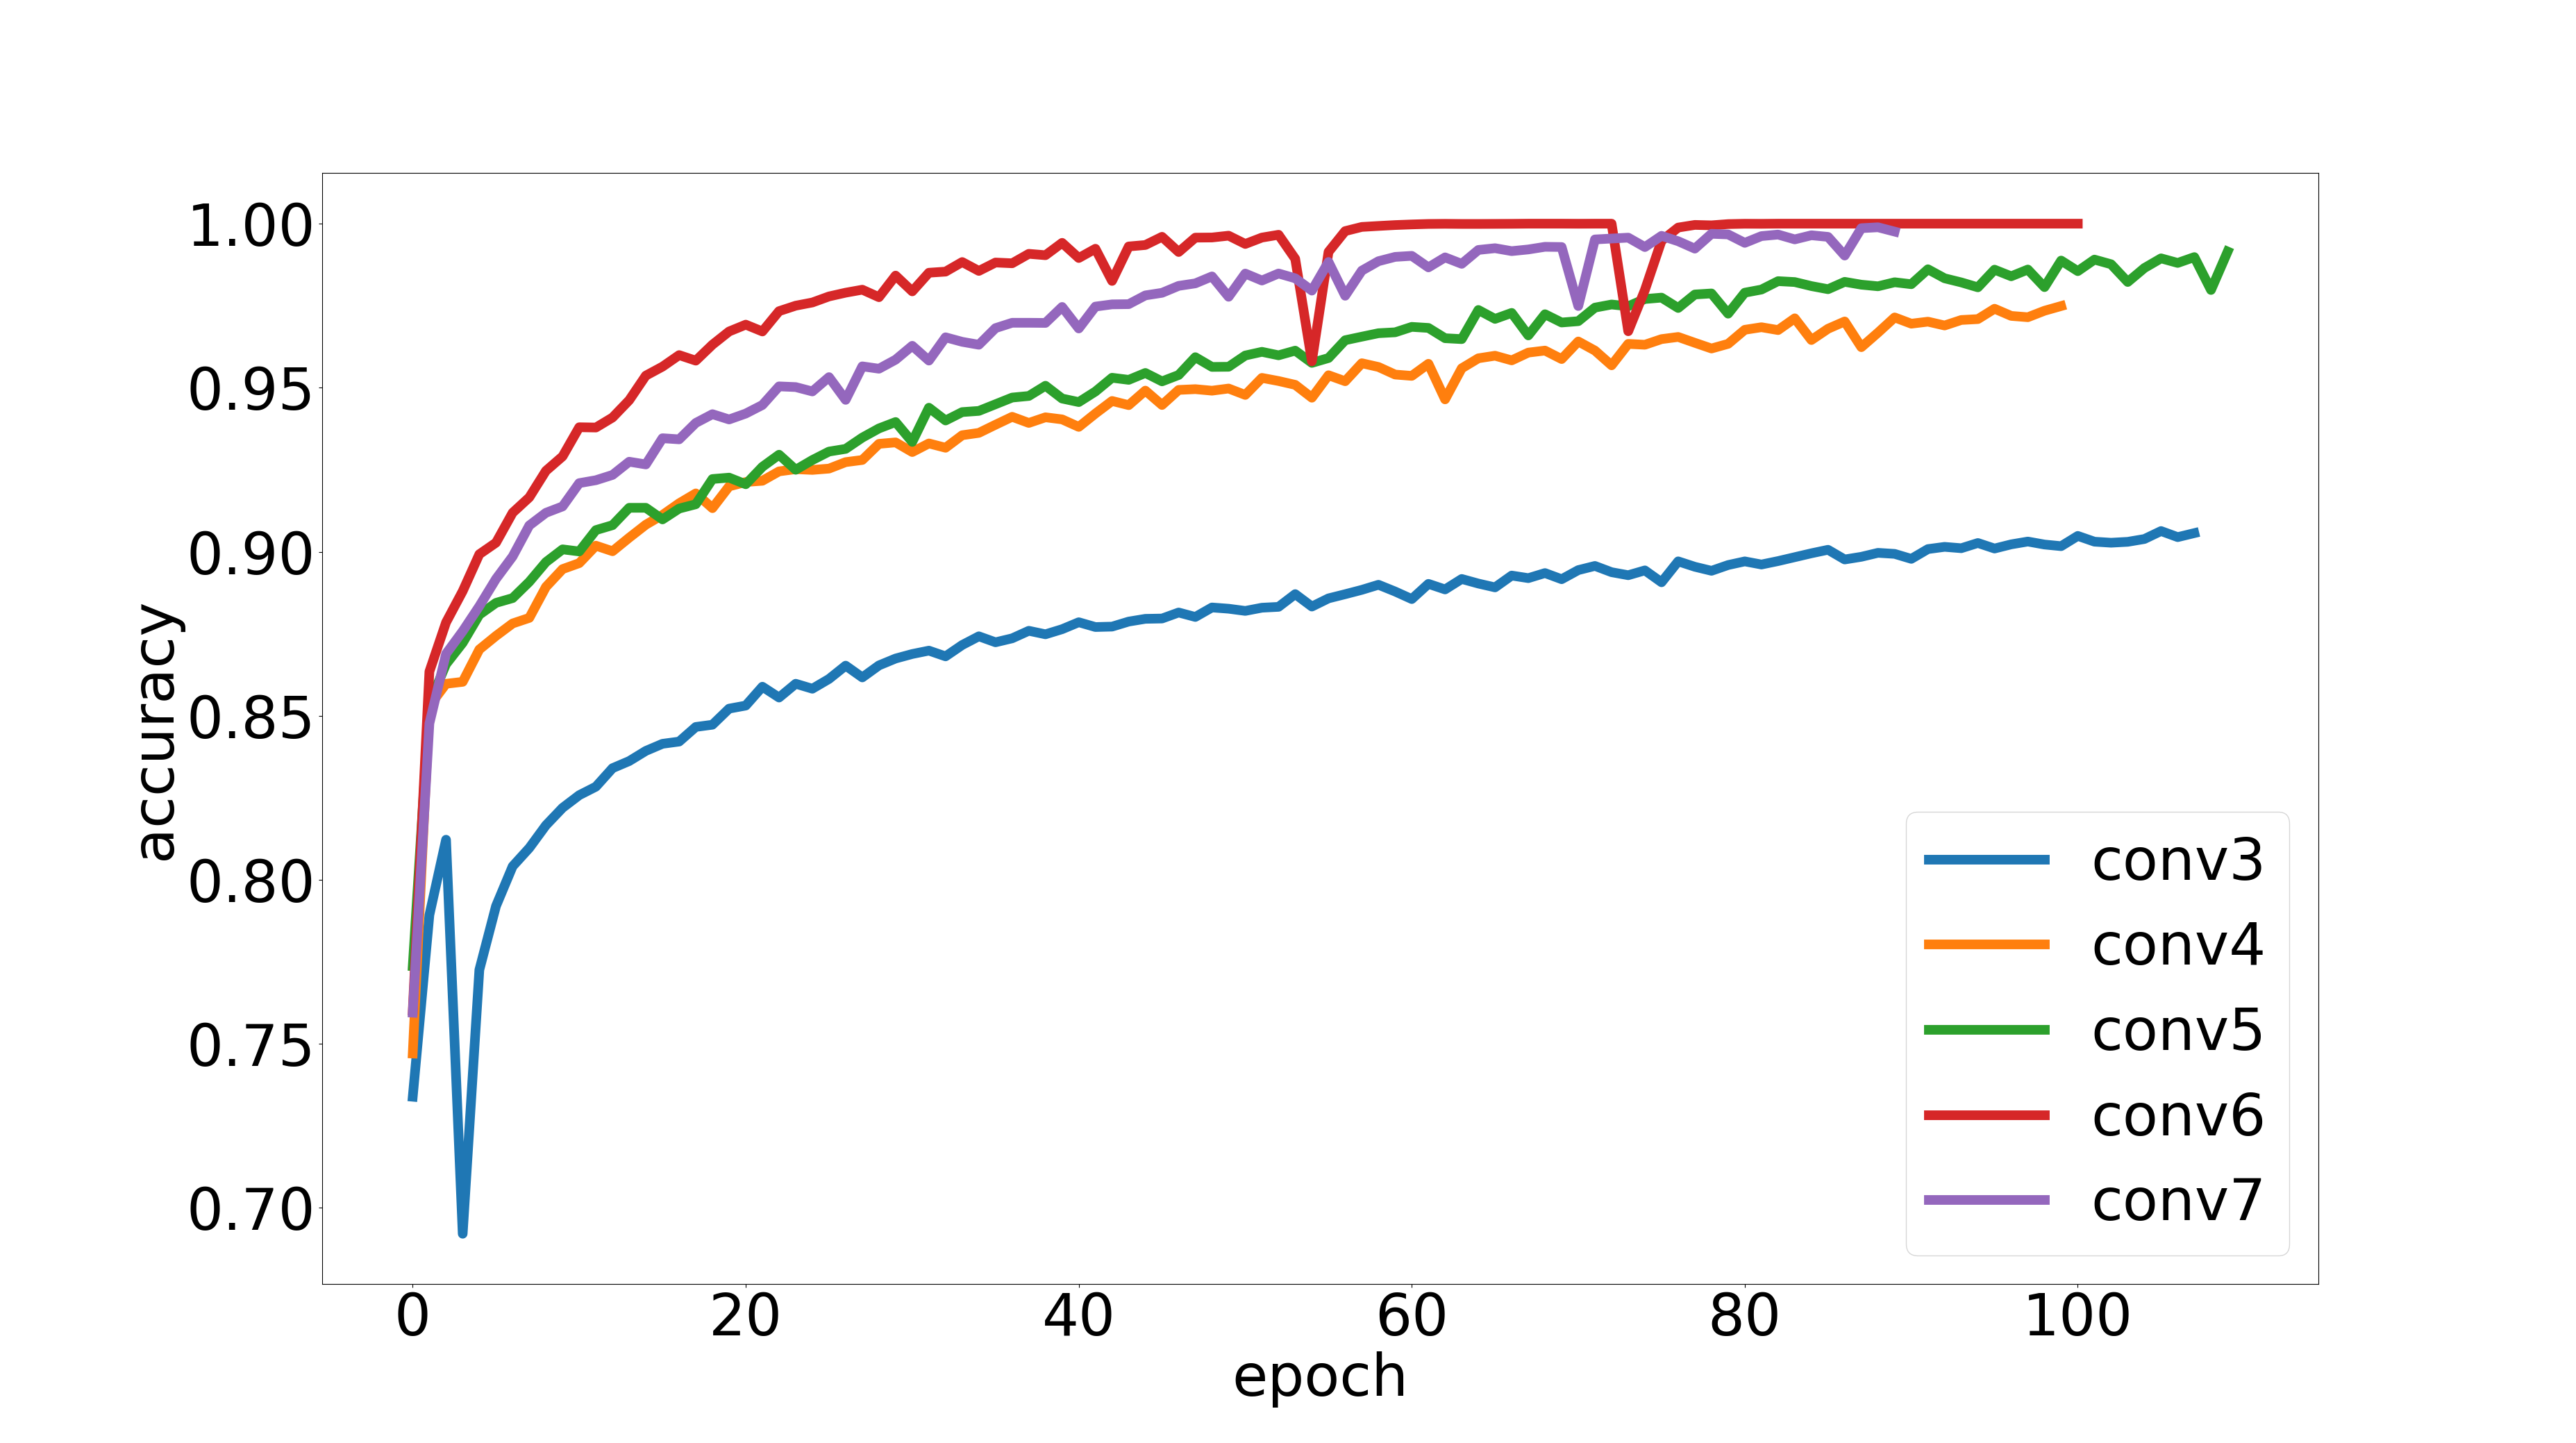
\includegraphics[width=55mm]{siameseLayers/train-acc.png}}\\
%\subfloat[Loss in validation]{\includegraphics[width=55mm]{siameseLayers/val-loss.png}}
%\subfloat[Accuracy in validation]{\includegraphics[width=55mm]{siameseLayers/val-acc.png}}
%
%
%
%\end{tabular}
%%\caption{Imatges MRI amb tumor.} \label{pseudo}
%\end{figure}
%
%
%\end{frame}

%\begin{frame}{CMC plot}
%
%
%
%\begin{figure}[hptb]
%\centering         
%\includegraphics[width=12cm]{siameseLayers/cmc2.png}
%%\caption{CMC plot.} \label{lossesSiam2}
%\end{figure}
%
%\end{frame}


\begin{frame}{Comparison reidentification methods}


\begin{figure}[hptb]
\centering         
\includegraphics[width=12cm]{siameseLayers/graps2.png}
%\caption{Performance-timing comparision.} \label{lossesSiam3}
\end{figure}

\end{frame}


\section{Validation experiments}


\begin{frame}{Results by sequence}

\begin{table}[!]
\centering

\resizebox{\textwidth}{!}{\begin{tabular}{l|llll|lll|ll|l}
                & \textbf{GT} & \textbf{MT} & \textbf{PT} & \textbf{ML} & \textbf{FP} & \textbf{FN} & \textbf{IDs}  & \textbf{MOTA} & \textbf{MOTP}  & \textbf{FPS} \\
\textit{02}     & 54          & 0           & 13          & 41          & 2181        & 15526       & 113                  & 0.1           & 67.1           & 9.02         \\
\textit{04}     & 83          & 0           & 41          & 42          & 5495        & 33980             & 290         & 16.6          & 71.1          &  12.3         \\
\textit{05}              & 125         & 3           & 43          & 79          & 28571       & 4713              & 109         & -12.2         & 67.8          & 17.94        \\
\textit{09}              & 25          & 1           & 19          & 5           & 932         & 3225              & 71          & 19.7          & 62           & 10.52        \\
\textit{10}              & 54          & 0           & 4           & 50          & 404         & 11647       & 81                    & 1.5           & 68.4                 & 14.23        \\
\textit{11}              & 69          & 0           & 16          & 53          & 948         & 7366        & 72                   & 8.6           & 71.4                 & 17.49        \\
\textit{13}              & 107         & 0           & 9           & 98          & 1315        & 10743       & 32                    & -5.6          & 67.1                  & 20.5         \\ \hline
\textit{Global} & 517         & 3           & 127         & 387         & 18896       & 78999       & 618                  & 10.8          & 70.3           & 15.85       
\end{tabular}}
\caption{Results algorithm by sequences.}
\label{tableResultsSequences}
\end{table}


\end{frame}

\begin{frame}{Weaknesses}

\begin{figure}[htbp]
\centering
\begin{tabular}{cc}
\subfloat[Hight texture blob]{\includegraphics[width=35mm]{texture/tomeuTetx.png}}
\subfloat[Low texture blob]{\includegraphics[width=35mm]{texture/donaTetx.png}}
\subfloat[Far away blob]{\includegraphics[width=35mm]{texture/foto004.png}}\\


\end{tabular}
%\caption{Imatges MRI amb tumor.} \label{pseudo}
\end{figure}

\end{frame}

%\begin{frame}{Example I}
%
%
%\begin{figure}[htbp]
%\centering
%\begin{tabular}{cc}
%\subfloat[Our]{\includegraphics[width=55mm]{comparision/our04.jpg}}
%\subfloat[Ground truth]{\includegraphics[width=55mm]{comparision/gt04.png}}\\
%
%
%
%
%\end{tabular}
%%\caption{Imatges MRI amb tumor.} \label{pseudo}
%\end{figure}
%
%\end{frame}
%
%
%
%\begin{frame}{Example II}
%
%
%\begin{figure}[htbp]
%\centering
%\begin{tabular}{cc}
%\subfloat[Our]{\includegraphics[width=55mm]{comparision/our09.jpg}}
%\subfloat[Ground truth]{\includegraphics[width=55mm]{comparision/gt09.png}}\\
%
%
%
%
%\end{tabular}
%%\caption{Imatges MRI amb tumor.} \label{pseudo}
%\end{figure}
%
%
%
%\end{frame}
%
%
%
%\begin{frame}{Example III}
%
%\begin{figure}[htbp]
%\centering
%\begin{tabular}{cc}
%\subfloat[Our]{\includegraphics[width=55mm]{comparision/our13.jpg}}
%\subfloat[Ground truth]{\includegraphics[width=55mm]{comparision/gt13.png}}\\
%
%
%
%
%\end{tabular}
%%\caption{Imatges MRI amb tumor.} \label{pseudo}
%\end{figure}
%
%
%\end{frame}

%
%\begin{frame}{Example IV}
%
%\begin{figure}[htbp]
%\centering
%\begin{tabular}{cc}
%\subfloat[Our]{\includegraphics[width=55mm]{comparision/our05.jpg}}
%\subfloat[Ground truth]{\includegraphics[width=55mm]{comparision/gt05.png}}\\
%
%
%
%
%\end{tabular}
%%\caption{Imatges MRI amb tumor.} \label{pseudo}
%\end{figure}
%
%
%\end{frame}

\begin{frame}{Comparison with SOTA}


\begin{figure}[hptb]
\centering         
\includegraphics[width=12cm]{comparision/timeDAta.png}
%\caption{Performance-timing comparision.} \label{lossesSiam3}
\end{figure}



\end{frame}


\begin{frame}{Timing performance I}

\begin{figure}[hptb]
\centering         
\includegraphics[width=12cm]{temps/figure4.png}
%\caption{Performance-timing comparision.} \label{lossesSiam3}
\end{figure}

\end{frame}

\begin{frame}{Timing performance II}

\begin{figure}[hptb]
\centering         
\includegraphics[width=12cm]{temps/framezomm4.png}
%\caption{Performance-timing comparision.} \label{lossesSiam3}
\end{figure}

\end{frame}

\section{Conclusions}


\begin{frame}{Conclusions}


\begin{itemize}

\item Object detector using deep learning.

\hspace{2cm}

\item Development of a Featured-based tracking module.

\hspace{2cm}

\item Merging detections and feature-based tracking, adding a reidentification module.

\hspace{2cm}

\item Testing of the component on an international databases.

\end{itemize}

\end{frame}



%\begin{frame}{Future work}
%
%
%\begin{itemize}
%
%\item Migration to C++.
%\item GPU implementation.
%
%\item Probabilistic framework.
%\item Improve siamese architectures. 
%
%\item Enhance data association.
%\end{itemize}
%
%
%\end{frame}

\begin{frame}

\hspace{2.3cm}
\Large
\textbf{Thank you for your attention !}

\begin{figure}[hptb]
\centering         
\includegraphics[width=5cm]{finale.png}
%\caption{Performance-timing comparision.} \label{lossesSiam3}
\end{figure}


\end{frame}

\end{document}



